% Created 2019-10-01 Tue 18:00
% Intended LaTeX compiler: pdflatex
\documentclass[11pt]{article}
\usepackage[utf8]{inputenc}
\usepackage[T1]{fontenc}
\usepackage{graphicx}
\usepackage{grffile}
\usepackage{longtable}
\usepackage{wrapfig}
\usepackage{rotating}
\usepackage[normalem]{ulem}
\usepackage{amsmath}
\usepackage{textcomp}
\usepackage{amssymb}
\usepackage{capt-of}
\usepackage{hyperref}
\usepackage{minted}
\usepackage[hyperref,x11names]{xcolor}
\usepackage{physics}
\usepackage{cases}
\graphicspath{ {./} }
\usepackage{tikz}
\usetikzlibrary{arrows,plotmarks,calc,positioning,fit}
\usetikzlibrary{shapes.geometric, decorations.pathmorphing, patterns, backgrounds}
\newcommand{\tikzremember}[1]{{  \tikz[remember picture,overlay]{\node (#1) at (0,11pt) { };}}}
\tikzset{snake it/.style={decorate, decoration=snake}}
\usepackage[nottoc]{tocbibind}
\author{Tigany Zarrouk}
\date{\today}
\title{PhD Log}
\hypersetup{
 pdfauthor={Tigany Zarrouk},
 pdftitle={PhD Log},
 pdfkeywords={},
 pdfsubject={},
 pdfcreator={Emacs 25.3.1 (Org mode 9.2.5)}, 
 pdflang={English}}
\begin{document}

\maketitle
\tableofcontents





\section{Tasks}
\label{sec:org27c6bbe}


\subsection{{\bfseries\sffamily TODO} Ti3Al report---DFT chapter}
\label{sec:orgd6e0e7b}
\begin{itemize}
\item Start with the theory of DFT with the HK theorem and KS equations to solve
for the density.
\item Talk a bit about the approximations that are made.
\item Alloy theory and the structure of Ti3Al
\item Look at literature to do with all of this. Go through why solutes are
incredibly important and why it is necessary do to this research.
\item How can solutes lead to failure and why is oxygen in particular bad for the alloy.
\item Is it wavy or planar slip
\item Go into the calculations and what I have done for them
\item Cite the research about the Fe and C vacancy concentration and what the
implications are for alloy research
\item What can I add to the research.
\end{itemize}
\subsection{{\bfseries\sffamily TODO} Ti/Ti3Al DFT oxygen interstitial/vacancy binding energy}
\label{sec:orge5f3942}
Want to find the vacancy formation energy, and the dissolution energy of
oxygen interstitials at different sites in the Ti3Al lattice. 

From these measurements we can then do a final calculation on the binding
energy of oxygen to a vacancy thus elucidating if it is favourable comapared
to just the normal positions. 

This will provide insight into the high amount of vacancies with oxygen. 
\subsubsection{Notes on the calculations}
\label{sec:orgbff9149}
\begin{enumerate}
\item Setting up relaxation
\label{sec:org3051925}
\begin{itemize}
\item To set up one calculates the self consistent density first by not initiating
\end{itemize}
relaxation. 

\begin{itemize}
\item Using the OPTIONS\textsubscript{HF} flag one can minimise the energy with respect to the
\end{itemize}
Harris-Foulkes energy, which is far faster. And it would use the initial
electron density for the relaxation, and then only calculate the density using
the overlap of atomic densities. 

One is then able to minimise the energy accordingly. 

\item Basis set optimisatons
\label{sec:orga65a295}

\begin{enumerate}
\item Notes on the basis set
\label{sec:org9792ae2}
It has been seen that the a smaller sphere radius for the oxygen was giving a much
larger overlap (\textasciitilde{}17\%) in the T2 interstitial site than any of the octahedral
sites, which have an overlap of \textasciitilde{}1.6\%. 

This would have decreased the accuracy of the results. 

So to decrease the radius of the oxygen and to increase the completeness of
the basis set one can introduce plane waves between certain energies such that
the plane wave basis set is more complete.

This should make the Harris-Foulkes energy smaller by the variational
principle. 

\textit{<2019-05-23 Thu 18:19>}

It seems that there is an optimal sphere radius of around 0.8. 
The best plane wave energy max seems to be at the maximum of around 3 Rydberg,
but this is at the edge of the range of search so it seems that the range
needs to be extended such that an optimum can be found before the basis set
becomes overcomplete. 

\textit{<2019-05-24 Fri 16:05>}

There seems to be an optimum. I shall stop putting the plane wave basis set up
in energy and now making pwemax = 4.0 ryd. 

The best sphere radius for the oxygen is 0.78.


\textit{<2019-05-24 Fri 18:01>}

Asking Dimitar about the plane wave basis set, he said to use the defaulf
values that are generated when making a blm file. 



\item Perfect lattice
\label{sec:org07f01ee}
spec name old rmax new rmax ratio 
1 Ti 2.707297 3.024213 1.117060 
2 Al 2.638772 2.947667 1.117060

Ti RSMH= 1.805 1.805 1.196 1.805 EH= -0.1 -0.1 -0.1 -0.1 
   RSMH2= 1.805 1.805 1.269 EH2= -0.9 -0.9 -0.9 P= 4.699 4.466 3.875 4.155 5.089 
Al RSMH= 1.759 1.759 1.352 EH= -0.1 -0.1 -0.1 
   RSMH2= 1.759 1.759 EH2= -0.9 -0.9 P= 3.837 3.75 3.392 4.13 5.089

gmax = 6.6

Ti RSMH= 1.805 1.805 1.269 1.805 EH= -0.1 -0.1 -0.1 -0.1 
   RSMH2= 1.805 1.805 1.269 EH2= -0.9 -0.9 -0.9 P= 4.699 4.466 3.875 4.155 5.089 
Al RSMH= 1.759 1.759 1.759 EH= -0.1 -0.1 -0.1 RSMH2= 1.759 1.759 EH2= -0.9 -0.9 P= 3.837 3.75 3.392 4.13 5.089

\item O2 site (least overlap)
\label{sec:orga8b1076}
spec name old rmax new rmax ratio 
1 Ti 2.663548 2.746597 1.031179 
2 Al 2.576718 2.746597 1.065928 
3 O 1.662251 1.714079 1.031179

Ti RSMH= 1.776 1.776 1.254 1.776 EH= -0.1 -0.1 -0.1 -0.1 RSMH2= 1.776 1.776 1.254 
   EH2= -0.9 -0.9 -0.9 P= 4.686 4.447 3.874 4.155 5.089 PZ= 0 13.9381 
Al RSMH= 1.718 1.718 1.718 EH= -0.1 -0.1 -0.1
   RSMH2= 1.718 1.718 EH2= -0.9 -0.9 P= 3.83 3.74 3.389 4.13 5.089 
O RSMH= 0.845 0.82 1.108 1.108 EH=-0.505 -0.1 -0.1 -0.1 RSMH2= 0.845 0.82 
   EH2= -1.305 -0.9 P= 2.886 2.858 3.25 4.11

\item O1 site (next least overlap)
\label{sec:org26e09b7}
spec name old rmax new rmax ratio 
1 Ti 2.641151 2.734882 1.035489 
2 Al 2.638731 3.547117 1.344251 
3 O 1.666646 1.725793 1.035489

gmax = 9.8
Ti RSMH= 1.761 1.761 1.246 1.761 EH= -0.1 -0.1 -0.1 -0.1 
   RSMH2= 1.761 1.761 1.246 EH2= -0.9 -0.9 -0.9 P= 4.679 4.437 3.873 4.155 5.089
   PZ= 0 13.9376 
Al RSMH= 1.759 1.759 1.759 EH= -0.1 -0.1 -0.1 
   RSMH2= 1.759 1.759 EH2= -0.9 -0.9 P=3.837 3.75 3.392 4.13 5.089 
O RSMH= 0.846 0.821 1.111 1.111 EH= -0.506 -0.1 -0.1 -0.1 RSMH2= 0.846 0.821
EH2= -1.306 -0.9 P= 2.886 2.859 3.25 4.11

\item T1 site (next most overlap)
\label{sec:org2f9342b}

spec name old rmax new rmax ratio 
1 Ti 2.654621 2.490980 0.938356 
2 Al 2.586159 2.447921 0.946547 
3 O 1.473639 1.382798 0.938356

gmax = 8.9

Ti RSMH= 1.77 1.77 1.251 1.77 EH= -0.1 -0.1 -0.1 -0.1 
   RSMH2= 1.77 1.77 1.251 EH2= -0.9 -0.9 -0.9 P= 4.683 4.443 3.874 4.155 5.089
   PZ= 0 13.9379 
Al RSMH=1.724 1.724 1.724 EH= -0.1 -0.1 -0.1 RSMH2= 1.724 1.724 EH2= -0.9 -0.9 
   P= 3.831 3.742 3.389 4.13 5.089 
O RSMH= 0.831 0.982 0.982 0.982 EH= -0.474 -0.1 -0.1 -0.1 RSMH2= 0.831 0.982 
  EH2= -1.274 -0.9 P= 2.871 2.845 3.25 4.11

\item T2 site (Most overlap)
\label{sec:org8ddc225}
\end{enumerate}
\end{enumerate}



\subsubsection{Vacancy formation energy definition}
\label{sec:org65d40ac}

\$\$ \(\Delta\) E\textsubscript{\text{f}}\textsuperscript{\text{vacancy}} = \(\lim\)\textsubscript{N\textsubscript{\text}\{a\} \(\to\) \(\infty\)} 
                                            \big$\backslash${E(N\textsubscript{\text}\{a\}, 1) 
\begin{itemize}
\item E(N\textsubscript{\text}\{a\} - 1, 0)   \big$\backslash$}  \$\$
\end{itemize}

Where the first argument of the energy function is the number of lattice sites
and the second denotes the number of vacancies. \cite{Finnis1997}

\subsubsection{Dissoluton energy of species definition}
\label{sec:org31af597}

The solution enthalpy of particular species is given by 

$$ E_{text{solution}} = E( \text{Ti}_{N}X_1 ) - E( \text{Ti}_{N}) - E( X ) $$

This is the same as  a formation energy \(\Delta E^{\text{f}}_{\text{O}}\)
\subsubsection{Vacancy-solute binding energy}
\label{sec:org17b98ea}
\cite{wolverton07_solut_vacan_bindin_alumin}

\$\$ -E\textsubscript{\text{bind}}( X - \text{Vac} ) = E( \text{Ti}\textsubscript{N - 2} X\textsubscript{1} \text{Vac}\textsubscript{1} )
\begin{itemize}
\item E( \text{Ti}\textsubscript{N})
\item E( \text{Ti}\textsubscript{N - 1} X\textsubscript{1} )
\item E( \text{Ti}\textsubscript{N - 1} \text{Vac}\textsubscript{1} ) \$\$
\end{itemize}

where Vac is a vacancy, X is a solute impurity. The binding energy is negative
here to keep with the convention that a \emph{positive} binding energy is
\emph{favourable}.

I think that there really is a minus sign here


\cite{deng16_ab_initio_solut_inter_impur}

\$\$ E\textsubscript{\text{bind}}\textsuperscript{V - X} =   + E( \text{Ti}\textsubscript{N - 1} X\textsubscript{1} ) 
\begin{itemize}
\item E( \text{Ti}\textsubscript{N - 1} \text{Vac}\textsubscript{1} )
\item E( \text{Ti}\textsubscript{N - 2} X\textsubscript{1} \text{Vac}\textsubscript{1} )
\item E( \text{Ti}\textsubscript{N})                       \$\$
\end{itemize}

\subsubsection{Dilute impurity energy and Vacancy formation energy}
\label{sec:orgb00ad0b}
\cite{wolverton07_solut_vacan_bindin_alumin}
\$\$ E\textsubscript{text\{impurity\}}(X) = E( \text{Ti}\textsubscript{N-1}X\textsubscript{1} ) 
\begin{itemize}
\item \frac{N-1}{N} E(\text{Ti}\textsubscript{N})
\item E( X ) \$\$
\end{itemize}

\$\$ E\textsubscript{text\{vacancy\}}(\text{Vac}) = E( \text{Ti}\textsubscript{N-1}\text{Vac}\textsubscript{1} ) 
\begin{itemize}
\item \frac{N-1}{N} E(\text{Ti}\textsubscript{N}) \$\$
\end{itemize}





\subsubsection{Basis set}
\label{sec:org5f84dfc}


\subsubsection{Relevant papers}
\label{sec:org9565b3c}
\cite{bakulin17_absor_diffus_oxygen_ti3al_alloy} 

\cite{wei11_effec_o_binar_phase_tial_ti3al_alloy}

\cite{bakulin18_effec_impur_format_energ_point}

\cite{mishin00_diffus_ti_al_system}

\cite{koizumi08_oxygen_diffus_ti3al_singl_cryst}




Koizumi states that there is a preference for the interstitial site that is O1
(6 Ti atom coordination). O2 sites (4 Ti \& 2 Al atom coordination), is of higher
energy. 

\begin{center}
\begin{tabular}{ll}
Site & Neighbouring atoms\\
\hline
O1 & 6 Ti\\
O2 & 4 Ti, 2 Al\\
T1 & 3 Ti, 1 Al (on Ti)\\
T2 & 3 Ti, 1 Al (on Al)\\
\end{tabular}
\end{center}

on Ti: the tetrahedral site is located just above a Ti atom in the c-axis direction.
on Al: the tetrahedral site is located just above an Al atom in the c-axis direction.



E\textsubscript{vacancy}\textsubscript{formation}
\begin{center}
\begin{tabular}{llrr}
Author & Geometry & V\textsubscript{Ti} & V\textsubscript{Al}\\
\hline
Baulkin (2018) & 2 x 2 x 2 & 2.209 & 2.894\\
Mishin  (2000) & Embedded atom? & 1.314 & 1.805\\
\end{tabular}
\end{center}


E\textsubscript{absorption} = - E\textsubscript{solution} 
The lower the solution the higher the binding energy 
the higher the absorption energy, the higher the binding energy. 

\begin{center}
\begin{tabular}{llrrrr}
Author & Geometry & O1 & O2 & T1 & T2\\
\hline
Wei     (2011) & Ti3Al/TiAl interface (6 \& 6 layers) & 6.23 & 4.75 & 4.20 & 3.83\\
Baulkin (2017) & 2 x 2 x 2 & 6.16 & 4.69 & 4.24 & 3.78\\
\end{tabular}
\end{center}

During relaxation it was found that the tetrahedral sites are unstable and
that they actually prefer the hexahedral sites (Baulkin). 

The chemical potential/diatomic reference energy for the oxygen molecule
decreases with increasing temperature. 
\begin{center}
\begin{tabular}{llrrrrrrrrr}
\hline
T & (K) & 0 & 500 & 1000 & 2000 & 2500 & 3000 & 4000 & 4500 & 5000\\
μO & (eV) & −4.35 & −4.89 & −5.5 & −6.83 & −7.54 & −8.27 & −9.78 & −10.55 & −11.34\\
\end{tabular}
\end{center}


\cite{hagen98_point_defec_chemic_poten_order_alloy}

Looked at point defects and soluted in an \(\text{A}_m\text{B}_n\) lattice. 

It is difficult to determine the concentrations of both vacancies and antisite
(substitutional of the other alloying element) defects reliably due to:
\begin{itemize}
\item Slow rates of diffusion -> Long equilibriation times.
\end{itemize}

Point-defect concentrations intimiately linked to chemical potentials of the
constituents, and these chemical potentials can be used to discuss relative
stability of different grain-boundary structures by comparing excess free
energies. 

We can say that there exists two sublattices, an A sublattice of \(m\) sites and a B
sublattice of \(n\) sites, with all atoms of a particular type only belonging to that
sublattice. 

The alloy deviates slightly from stochiometry so we have
\(\text{A}_{x}\text{B}_{1-x}\) where we suppose \(x\) to be within a few percent
of \(m/(m+n)\). Each site of each sublattice can by occupied by its own atom or
an atom of the other kind or a vacancy.

\(c_{aa}\) = concentration of A atoms on the A sublattice; 
\(c_{bb}\) = concentration of B atoms on the B sublattice;        
\(c_{ab}\) = concentration of A atoms on the B sublattice;       
\(c_{ba}\) = concentration of B atoms on the A sublattice;       
\(c_{va}\) = concentration of vacancies on the A sublattice;     
\(c_{vb}\) = concentration of vacancies on the B sublattice.

Number of A and B sublattice cites are \(Nm\) and \(Nn\). \(N\) is the number of
fomulae units, which can vary due to the creation/annihilation of vacancies
when the temperature or stochiometry varies, while the ratio \(m/n\) is
constant. 

A canonical ensemble is assumed so that the total numbers of A and B atoms are
conserved. 

There are 7 unknowns in a statistical model of the concentrations, \(c_i\) and
\(N\) and they satisfy the constraints 

\[ c_{aa} + c_{ba} + c_{va} = 1  \] 
\[ c_{bb} + c_{ab} + c_{vb} = 1  \]

There are fixed numbers \(n_a\) and \(n_b\) of A and B atoms are given by 

\[ N ( m c_{aa}  +  n c_{ab} )  =  n_a \]
\[ N ( m c_{ba}  +  n c_{bb} )  =  n_b \]

There are seven unknowns and four equations so there are three independent
variables. The conservation of atoms constrains the possible defects which can
be generated thermally. The effect of possible defect clustering or ordering
is not included. 


For a material of a single element, the calculation of, for example, the
vacancy formation energy is simple: calculate the total energy of a perfect
lattice and subtract it from the energy of a lattice with a defect. This is
unique if \(N\) is sufficiently large and \emph{the same number of atoms is compared}
with and without the defect. 

For an ordered alloy the stochiometry comes into account, so it is not as
simple. The physical consequences, of having a working definition, are that we
take the equilibrium concentrations of the four point defects and that they
must be independent of the definition adoped for the point-defect energies, as
long as the formulation is consistent. 

If all we want at the end of the calcuation are the equilibrium point-defect
concentrations, we do not need single point-defect energies, but rather the
energies of threee independent stociometry-conserving complex defects. For
example it is possible to compare the energy of a block AB containing a pair of
vacancies or a triple defect with the energy of the same numbers of A and B
atoms in a perfect crystal. However the above uniquely defined complex defect
energies can be constructed simple from calculations of individual point-deect
energies. 


\(e_{\text{mol}}\): Cohesive energy / energy per unit mole.  
We can arbitrariliy divide this between atoms of A and B type. This is a
natural division in EAM potentials or BOP potentials which allocate energies to
each atom. 

\[ e_{\text{mol}} = m e_{aa} + n e_{bb}  \]

The energy of a block containing \(Nm\) sites of sublattice A and \(Nn\) sites of
sublattice B is now:


$\backslash$[ E = Nm ( c\textsubscript{aa} e\textsubscript{aa} + c\textsubscript{ba} e\textsubscript{ba} + c\textsubscript{va} e\textsubscript{va} ) 
\begin{itemize}
\item Nn ( c\textsubscript{bb} e\textsubscript{bb} + c\textsubscript{ab} e\textsubscript{ab} + c\textsubscript{vb} e\textsubscript{vb} ) $\backslash$]
\end{itemize}

The assumption has been made that the point defects are assumed to be
sufficiently dilute that interactions may be neglected. 

We can caw calculate the formation energy \(e_{vb}\) of a B vacancy. Construct
block of \(N\) formula units with \(Nm\) sites of A, fully occupies by type A
atoms, and \(Nn - 1\) sites of type B with a vacancy on the remaining site.

\[ e_{vb} = E(N, vb) - Nm e_{aa} - ( Nn - 1 ) e_{bb} \]

The energy of an A antisite is:
\[ e_{ab} = E(N, ab) - Nm e_{aa} - ( Nn - 1 ) e_{bb} \]

One can define stochiometry-conserving complexes (in the case of NiAl) 

\[ e_{2v} =   e_{va} + e_{vb} \]
\[ e_{ta} = 2 e_{vb} + e_{ba} - e_{bb} \]
\[ e_{tb} = 2 e_{va} + e_{ab} - e_{aa} \]

This formalism can be generalised to finite temperature if for \emph{energy} we read
\emph{free energy} and the include both the vibrational entropy and the effect of
temperature on the formation energies. (We are not including configurational
entropy at this stage). Essentially one can do phonon calculations and then
obtain the entropy from standard formulae. The effect is to add \(- Ts_i\) to
each of the \(e_i\).


To find the enthalpy of the defected crystal, neglecting elastic strains, the
total volume can be written as 

$\backslash$[ V = Nm ( c\textsubscript{aa} \(\Omega\)\textsubscript{aa} + c\textsubscript{ba} \(\Omega\)\textsubscript{ba} + c\textsubscript{va} \(\Omega\)\textsubscript{va} ) 
\begin{itemize}
\item Nn ( c\textsubscript{bb} \(\Omega\)\textsubscript{bb} + c\textsubscript{ab} \(\Omega\)\textsubscript{ab} + c\textsubscript{vb} \(\Omega\)\textsubscript{vb} ) $\backslash$]
\end{itemize}

where \(\Omega_i\) are the partial molar volume and the quantity \(m\Omega_{aa} +
n\Omega_{bb}\) is uniquely defined as the volume per formula unit, but like the
energies this is arbitrarily defined between A and B. 


Relaxation volumes are uniquely defined, like that of a B vacancy:
\[ \Omega_{bb} - \Omega_{vb} = N( m \Omega_{aa} + n \Omega_{bb} ) - V(N,vb)  \]

where \(V(N,vb)\) is the volume of a crystal with \(N\) formula units with a single
vacancy of the B sublattice. 

Adding the \(pV\) term to construc the enthalpy amounts to replacing \(e_i\) by
\(e_i + p\Omega_i\) everywhere. The total Gibbs free energy without the
configurational part is therefore given by replacing each of the \(e_i\) in the
equations for \(e_{vb}\) and \(e_{ab}\) with \(e_i + p\Omega_i - T s_i\). These
pressure and entropy terms are not included in the following for simplicity but
they can be included. 

The configurational entropy of the model system is 

$\backslash$[ S = Nmk ( c\textsubscript{aa} \text{log} c\textsubscript{aa} + c\textsubscript{ba} \text{log} c\textsubscript{ba} + c\textsubscript{va} \text{log} c\textsubscript{va} ) 
\begin{itemize}
\item Nnk ( c\textsubscript{bb} \text{log} c\textsubscript{bb} + c\textsubscript{ab} \text{log} c\textsubscript{ab} + c\textsubscript{vb} \text{log} c\textsubscript{vb} ) $\backslash$]
\end{itemize}

\subsection{{\bfseries\sffamily TODO} Write up fitting and optimisation}
\label{sec:org5790233}
\begin{itemize}
\item Used Genetic Algorithm and CMAES.
\item Add in quantities to fit to.
\end{itemize}


\begin{itemize}
\item Realised that the prismatic fault was not high enough.
\end{itemize}

This caused incredibly large dissociation along the prismatic plane for a
screw dislocation. 

This was unreasonable, and it has been assumed that this can be rectified by a
short ranged, very quickly decaying power law added to the pair potential. 

Although this means that we need a refitting of the pair potential. 

Unfortunately it seems that the accordance with the DFT results of the
correct energetic ordering of the phases is lost: omega phase is \textbf{not}
lower in energy than that of the hcp phase.


Reasonable starting point is:

PARAMETERS
  b2=60204900.7590034157 m2=-13.7544131202 p2=0.0000000000 fdd=0.2648249504 qdds=0.5697753882 qddp=0.5648597117 qddd=0.8213593849 b0=49.7557565400 p0=1.1050685730 b1=-5.097
3416100 p1=0.6991977165 ndt=2.0000000000 cr1=-6.0000000000 cr2=3.2217589360 r1dd=6.5000000000 rcdd=10.0000000000 cr3=-1.1418272350 rmaxhm=10.1000000000 npar=18 
VARGS
    -vb2=60204900.7590034157 -vm2=-13.7544131202 -vp2=0.0000000000 -vfdd=0.2648249504 -vqdds=0.5697753882 -vqddp=0.5648597117 -vqddd=0.8213593849 -vb0=49.7557565400 -vp0=1.
1050685730 -vb1=-5.0973416100 -vp1=0.6991977165 -vndt=2.0000000000 -vcr1=-6.0000000000 -vcr2=3.2217589360 -vr1dd=6.5000000000 -vrcdd=10.0000000000 -vcr3=-1.1418272350 -vrma
xhm=10.1000000000 

Quantity      predicted    target     norm\textsubscript{pred}   norm\textsubscript{tar}    sq diff.      weight    objective * 100\textsuperscript{2} 

\noindent\rule{\textwidth}{0.5pt}
a\textsubscript{hcp}   :   5.69823736   5.57678969   5.69823736   5.57678969   0.01474954 1000.00000000    147495.36
c/a     :   1.57540221   1.58731122  15.29618259  15.41181168   0.01337009 100.00000000     13370.09
a\textsubscript{omega} :   9.11713244   8.73254342   1.13964156   1.09156793   0.00231107  10.00000000       231.11
c\textsubscript{omega} :   5.50357270   5.32343103   0.68794659   0.66542888   0.00050705  10.00000000        50.70
a\textsubscript{4h}    :   5.68949374   5.56325146   1.02269218   1.00000000   0.00051493   1.00000000         5.15
c\textsubscript{4h}    :  18.46292975  17.75908031   1.03963321   1.00000000   0.00157079   1.00000000        15.71
a\textsubscript{6h}    :   5.68593900   5.54639384   1.02515962   1.00000000   0.00063301   1.00000000         6.33
c\textsubscript{6h}    :  27.74967218  26.77136353   1.03654310   1.00000000   0.00133540   1.00000000        13.35
a\textsubscript{bcc}   :   6.20079768   6.17948863   0.88582824   0.88278409   0.00000927   1.00000000         0.09
a\textsubscript{fcc}   :   8.03310655   7.88677000   1.14758665   1.12668143   0.00043703   1.00000000         4.37
DE(o,h) :   1.19189500  -0.63343333   0.07945967  -0.04222889   0.01480810 3000.00000000    444243.14
DE(4h,h):   1.83337000   3.17160000   0.00733348   0.01268640   0.00002865 2000.00000000       573.08
DE(6h,h):   2.75695000   3.72005000   0.01102780   0.01488020   0.00001484 2000.00000000       296.82
DE(b,h) :   9.39020500   7.63520000   0.09485056   0.07712323   0.00031426   1.00000000         3.14
DE(f,h) :   4.17199500   4.51880000   0.04214136   0.04564444   0.00001227 2000.00000000       245.43
c\textsubscript{11}    : 211.10292175 176.10000000   0.92212869   0.76923077   0.02337778 100.00000000     23377.78
c\textsubscript{33}    : 232.93926611 190.50000000   0.94059869   0.76923077   0.02936697 100.00000000     29366.97
c\textsubscript{44}    :  55.49057353  50.80000000   0.84025702   0.76923077   0.00504473 100.00000000      5044.73
c\textsubscript{12}    : 110.56430372  86.90000000   0.97870500   0.76923077   0.04387945 100.00000000     43879.45
c\textsubscript{13}    :  73.53441848  68.30000000   0.82818356   0.76923077   0.00347543  10.00000000       347.54
M\textsubscript{freq}\textsubscript{0}:   2.86541811   2.85858719   0.20883117   0.20833333   0.00000025   0.10000000         0.00
M\textsubscript{freq}\textsubscript{1}:   2.86541812   2.85858719   0.20883117   0.20833333   0.00000025   0.10000000         0.00
M\textsubscript{freq}\textsubscript{2}:   2.86541812   2.85858719   0.20883117   0.20833333   0.00000025   0.10000000         0.00
M\textsubscript{freq}\textsubscript{3}:   2.86541813   2.85858719   0.20883117   0.20833333   0.00000025   0.10000000         0.00
M\textsubscript{freq}\textsubscript{4}:   6.16074486   5.66706047   0.22648223   0.20833333   0.00032938   0.10000000         0.33
M\textsubscript{freq}\textsubscript{5}:   6.16074486   5.66706047   0.22648223   0.20833333   0.00032938   0.10000000         0.33
H\textsubscript{freq}\textsubscript{0}:   4.29880135   4.80643423   0.18633015   0.20833333   0.00048414   0.10000000         0.48
H\textsubscript{freq}\textsubscript{1}:   4.29880135   5.58010025   0.16049597   0.20833333   0.00228841   0.10000000         2.29
H\textsubscript{freq}\textsubscript{2}:   6.76073943   5.65316738   0.24915013   0.20833333   0.00166601   0.10000000         1.67
H\textsubscript{freq}\textsubscript{3}:   6.76073943   6.36651842   0.22123354   0.20833333   0.00016642   0.10000000         0.17
H\textsubscript{freq}\textsubscript{4}:   8.32761036   6.40050186   0.27105981   0.20833333   0.00393461   0.10000000         3.93
H\textsubscript{freq}\textsubscript{5}:   8.32761036   7.64082373   0.22705913   0.20833333   0.00035066   0.10000000         0.35
bandw. G:   4.58784139   5.87085872   1.30243337   1.66666667   0.13266589  15.00000000     19899.88
bandw. K:   5.68718179   4.97424321   1.03938731   0.90909091   0.01697715  15.00000000      2546.57
bandw. M:   6.52257165   7.78109872   1.39709740   1.66666667   0.07266759  15.00000000     10900.14
bandw. L:   5.25996287   6.34433701   1.38179999   1.66666667   0.08114903  15.00000000     12172.35
bandw. H:   4.39872218   9.70902614   0.41186812   0.90909091   0.24723050   5.00000000     12361.53
DOSerr\textsubscript{h}:   0.00000000   0.00000000   0.00000000   0.00000000   0.00000000   1.00000000         0.00
DOSerr\textsubscript{o}:  95.30342229   0.00000000  95.30342229   0.00000000 9082.74230017   0.00000000         0.00
E\textsubscript{pris}\textsubscript{f}: 119.59113352 220.00000000 119.59113352 220.00000000 10081.94046857 100000.00000000 10081940468565.85





PARAMETERS
  b2=73362700.7877650857 m2=-13.9508390550 p2=0.0000000000 fdd=0.2648249504 qdds=0.5697753882 qddp=0.5648597117 qddd=0.8213593849 b0=49.7557565400 p0=1.1050685730 b1=-5.097
3416100 p1=0.6991977165 ndt=2.0000000000 cr1=-6.0000000000 cr2=3.2217589360 r1dd=6.5000000000 rcdd=10.0000000000 cr3=-1.1418272350 rmaxhm=10.1000000000 npar=18 
VARGS
    -vb2=73362700.7877650857 -vm2=-13.9508390550 -vp2=0.0000000000 -vfdd=0.2648249504 -vqdds=0.5697753882 -vqddp=0.5648597117 -vqddd=0.8213593849 -vb0=49.7557565400 -vp0=1.
1050685730 -vb1=-5.0973416100 -vp1=0.6991977165 -vndt=2.0000000000 -vcr1=-6.0000000000 -vcr2=3.2217589360 -vr1dd=6.5000000000 -vrcdd=10.0000000000 -vcr3=-1.1418272350 -vrma
xhm=10.1000000000 

Quantity      predicted    target     norm\textsubscript{pred}   norm\textsubscript{tar}    sq diff.      weight    objective * 100\textsuperscript{2} 

\noindent\rule{\textwidth}{0.5pt}
a\textsubscript{hcp}   :   5.68326063   5.57678969   5.68326063   5.57678969   0.01133606 1000.00000000    113360.60
c/a     :   1.58164523   1.58731122  15.35679851  15.41181168   0.00302645 100.00000000      3026.45
a\textsubscript{omega} :   9.09093887   8.73254342   1.13636736   1.09156793   0.00200699  10.00000000       200.70
c\textsubscript{omega} :   5.49075443   5.32343103   0.68634430   0.66542888   0.00043745  10.00000000        43.75
a\textsubscript{4h}    :   5.67495771   5.56325146   1.02007931   1.00000000   0.00040318   1.00000000         4.03
c\textsubscript{4h}    :  18.41194892  17.75908031   1.03676252   1.00000000   0.00135148   1.00000000        13.51
a\textsubscript{6h}    :   5.67118026   5.54639384   1.02249866   1.00000000   0.00050619   1.00000000         5.06
c\textsubscript{6h}    :  27.67479817  26.77136353   1.03374631   1.00000000   0.00113881   1.00000000        11.39
a\textsubscript{bcc}   :   6.20079768   6.17948863   0.88582824   0.88278409   0.00000927   1.00000000         0.09
a\textsubscript{fcc}   :   8.01192626   7.88677000   1.14456089   1.12668143   0.00031968   1.00000000         3.20
DE(o,h) :   1.09675833  -0.63343333   0.07311722  -0.04222889   0.01330473 3000.00000000    399141.76
DE(4h,h):   1.84836500   3.17160000   0.00739346   0.01268640   0.00002802 2000.00000000       560.30
DE(6h,h):   2.77866667   3.72005000   0.01111467   0.01488020   0.00001418 2000.00000000       283.58
DE(b,h) :   8.85897500   7.63520000   0.08948460   0.07712323   0.00015280   1.00000000         1.53
DE(f,h) :   4.20064500   4.51880000   0.04243076   0.04564444   0.00001033 2000.00000000       206.56
c\textsubscript{11}    : 209.98522208 176.10000000   0.91724642   0.76923077   0.02190863 100.00000000     21908.63
c\textsubscript{33}    : 232.98310764 190.50000000   0.94077572   0.76923077   0.02942767 100.00000000     29427.67
c\textsubscript{44}    :  54.68686450  50.80000000   0.82808699   0.76923077   0.00346405 100.00000000      3464.05
c\textsubscript{12}    : 109.06955946  86.90000000   0.96547366   0.76923077   0.03851127 100.00000000     38511.27
c\textsubscript{13}    :  73.74195452  68.30000000   0.83052094   0.76923077   0.00375649  10.00000000       375.65
M\textsubscript{freq}\textsubscript{0}:   2.85519402   2.85858719   0.20808604   0.20833333   0.00000006   0.10000000         0.00
M\textsubscript{freq}\textsubscript{1}:   2.85519403   2.85858719   0.20808604   0.20833333   0.00000006   0.10000000         0.00
M\textsubscript{freq}\textsubscript{2}:   2.85519403   2.85858719   0.20808604   0.20833333   0.00000006   0.10000000         0.00
M\textsubscript{freq}\textsubscript{3}:   2.85519404   2.85858719   0.20808604   0.20833333   0.00000006   0.10000000         0.00
M\textsubscript{freq}\textsubscript{4}:   6.14081288   5.66706047   0.22574949   0.20833333   0.00030332   0.10000000         0.30
M\textsubscript{freq}\textsubscript{5}:   6.14081288   5.66706047   0.22574949   0.20833333   0.00030332   0.10000000         0.30
H\textsubscript{freq}\textsubscript{0}:   4.24870561   4.80643423   0.18415877   0.20833333   0.00058441   0.10000000         0.58
H\textsubscript{freq}\textsubscript{1}:   4.24870561   5.58010025   0.15862565   0.20833333   0.00247085   0.10000000         2.47
H\textsubscript{freq}\textsubscript{2}:   6.73808691   5.65316738   0.24831533   0.20833333   0.00159856   0.10000000         1.60
H\textsubscript{freq}\textsubscript{3}:   6.73808691   6.36651842   0.22049227   0.20833333   0.00014784   0.10000000         0.15
H\textsubscript{freq}\textsubscript{4}:   8.32193375   6.40050186   0.27087504   0.20833333   0.00391147   0.10000000         3.91
H\textsubscript{freq}\textsubscript{5}:   8.32193375   7.64082373   0.22690436   0.20833333   0.00034488   0.10000000         0.34
bandw. G:   4.63954304   5.87085872   1.31711085   1.66666667   0.12218927  15.00000000     18328.39
bandw. K:   5.74840743   4.97424321   1.05057689   0.90909091   0.02001828  15.00000000      3002.74
bandw. M:   6.57699445   7.78109872   1.40875444   1.66666667   0.06651871  15.00000000      9977.81
bandw. L:   5.31166452   6.34433701   1.39538209   1.66666667   0.07359532  15.00000000     11039.30
bandw. H:   4.44226042   9.70902614   0.41594476   0.90909091   0.24319312   5.00000000     12159.66
DOSerr\textsubscript{h}:   0.00000000   0.00000000   0.00000000   0.00000000   0.00000000   1.00000000         0.00
DOSerr\textsubscript{o}:  98.57124703   0.00000000  98.57124703   0.00000000 9716.29074056   0.00000000         0.00
E\textsubscript{pris}\textsubscript{f}: 119.88060210 220.00000000 119.88060210 220.00000000 10023.89383558 100000.00000000 10023893835581.32



  b2=91394018.8920019716 m2=-14.4689417704 p2=0.0000000000 fdd=0.2648249504 qdds=0.5697753882 qddp=0.5648597117 qddd=0.8213593849 b0=49.7557565400 p0=1.1050685730 b1=-5.097
3416100 p1=0.6991977165 ndt=2.0000000000 cr1=-6.0000000000 cr2=3.2217589360 r1dd=6.5000000000 rcdd=10.0000000000 cr3=-1.1418272350 rmaxhm=10.1000000000 npar=18 
VARGS
    -vb2=91394018.8920019716 -vm2=-14.4689417704 -vp2=0.0000000000 -vfdd=0.2648249504 -vqdds=0.5697753882 -vqddp=0.5648597117 -vqddd=0.8213593849 -vb0=49.7557565400 -vp0=1.
1050685730 -vb1=-5.0973416100 -vp1=0.6991977165 -vndt=2.0000000000 -vcr1=-6.0000000000 -vcr2=3.2217589360 -vr1dd=6.5000000000 -vrcdd=10.0000000000 -vcr3=-1.1418272350 -vrma
xhm=10.1000000000 

Quantity      predicted    target     norm\textsubscript{pred}   norm\textsubscript{tar}    sq diff.      weight    objective * 100\textsuperscript{2} 

\noindent\rule{\textwidth}{0.5pt}
a\textsubscript{hcp}   :   5.62525983   5.57678969   5.62525983   5.57678969   0.00234935 1000.00000000     23493.55
c/a     :   1.60613643   1.58731122  15.59459288  15.41181168   0.03340896 100.00000000     33408.96
a\textsubscript{omega} :   8.98530887   8.73254342   1.12316361   1.09156793   0.00099829  10.00000000        99.83
c\textsubscript{omega} :   5.44549052   5.32343103   0.68068632   0.66542888   0.00023279  10.00000000        23.28
a\textsubscript{4h}    :   5.61807095   5.56325146   1.00985386   1.00000000   0.00009710   1.00000000         0.97
c\textsubscript{4h}    :  18.21768083  17.75908031   1.02582344   1.00000000   0.00066685   1.00000000         6.67
a\textsubscript{6h}    :   5.61365761   5.54639384   1.01212748   1.00000000   0.00014708   1.00000000         1.47
c\textsubscript{6h}    :  27.38802263  26.77136353   1.02303428   1.00000000   0.00053058   1.00000000         5.31
a\textsubscript{bcc}   :   6.20079768   6.17948863   0.88582824   0.88278409   0.00000927   1.00000000         0.09
a\textsubscript{fcc}   :   7.93028587   7.88677000   1.13289798   1.12668143   0.00003865   1.00000000         0.39
DE(o,h) :   0.56552167  -0.63343333   0.03770144  -0.04222889   0.00638886 3000.00000000    191665.75
DE(4h,h):   1.90610750   3.17160000   0.00762443   0.01268640   0.00002562 2000.00000000       512.47
DE(6h,h):   2.86158833   3.72005000   0.01144635   0.01488020   0.00001179 2000.00000000       235.83
DE(b,h) :   7.52522500   7.63520000   0.07601237   0.07712323   0.00000123   1.00000000         0.01
DE(f,h) :   4.31089500   4.51880000   0.04354439   0.04564444   0.00000441 2000.00000000        88.20
c\textsubscript{11}    : 199.90553801 176.10000000   0.87321687   0.76923077   0.01081311 100.00000000     10813.11
c\textsubscript{33}    : 226.98933014 190.50000000   0.91657311   0.76923077   0.02170976 100.00000000     21709.76
c\textsubscript{44}    :  52.69685443  50.80000000   0.79795358   0.76923077   0.00082500 100.00000000       825.00
c\textsubscript{12}    :  98.48673287  86.90000000   0.87179546   0.76923077   0.01051952 100.00000000     10519.52
c\textsubscript{13}    :  72.19938307  68.30000000   0.81314769   0.76923077   0.00192870  10.00000000       192.87
M\textsubscript{freq}\textsubscript{0}:   2.78990046   2.85858719   0.20332746   0.20833333   0.00002506   0.10000000         0.03
M\textsubscript{freq}\textsubscript{1}:   2.78990047   2.85858719   0.20332746   0.20833333   0.00002506   0.10000000         0.03
M\textsubscript{freq}\textsubscript{2}:   2.78990047   2.85858719   0.20332746   0.20833333   0.00002506   0.10000000         0.03
M\textsubscript{freq}\textsubscript{3}:   2.78990048   2.85858719   0.20332746   0.20833333   0.00002506   0.10000000         0.03
M\textsubscript{freq}\textsubscript{4}:   6.00974100   5.66706047   0.22093101   0.20833333   0.00015870   0.10000000         0.16
M\textsubscript{freq}\textsubscript{5}:   6.00974100   5.66706047   0.22093101   0.20833333   0.00015870   0.10000000         0.16
H\textsubscript{freq}\textsubscript{0}:   3.99826489   4.80643423   0.17330350   0.20833333   0.00122709   0.10000000         1.23
H\textsubscript{freq}\textsubscript{1}:   3.99826489   5.58010025   0.14927543   0.20833333   0.00348784   0.10000000         3.49
H\textsubscript{freq}\textsubscript{2}:   6.58970446   5.65316738   0.24284706   0.20833333   0.00119120   0.10000000         1.19
H\textsubscript{freq}\textsubscript{3}:   6.58970446   6.36651842   0.21563671   0.20833333   0.00005334   0.10000000         0.05
H\textsubscript{freq}\textsubscript{4}:   8.23482251   6.40050186   0.26803961   0.20833333   0.00356484   0.10000000         3.56
H\textsubscript{freq}\textsubscript{5}:   8.23482251   7.64082373   0.22452920   0.20833333   0.00026231   0.10000000         0.26
bandw. G:   4.85043136   5.87085872   1.37697953   1.66666667   0.08391864  15.00000000     12587.80
bandw. K:   5.99194943   4.97424321   1.09508653   0.90909091   0.03459437  15.00000000      5189.16
bandw. M:   6.79332504   7.78109872   1.45509122   1.66666667   0.04476417  15.00000000      6714.63
bandw. L:   5.51847114   6.34433701   1.44971049   1.66666667   0.04706998  15.00000000      7060.50
bandw. H:   4.61097107   9.70902614   0.43174174   0.90909091   0.22786222   5.00000000     11393.11
DOSerr\textsubscript{h}:   0.00000000   0.00000000   0.00000000   0.00000000   0.00000000   1.00000000         0.00
DOSerr\textsubscript{o}: 111.68287062   0.00000000 111.68287062   0.00000000 12473.06358905   0.00000000         0.00
E\textsubscript{pris}\textsubscript{f}: 105.39637060 220.00000000 105.39637060 220.00000000 13133.99187172 100000.00000000 13133991871718.04


PARAMETERS
  b2=901772799.4098891020 m2=-15.7042290440 p2=0.0000000000 fdd=0.2648249504 qdds=0.5697753882 qddp=0.5648597117 qddd=0.8213593849 b0=47.9215925588 p0=1.1092837121 b1=-3.99
59790920 p1=0.6574344463 ndt=2.0000000000 cr1=-6.0000000000 cr2=3.2217589360 r1dd=6.5000000000 rcdd=10.0000000000 cr3=-1.1418272350 rmaxhm=10.1000000000 npar=18 
VARGS
    -vb2=901772799.4098891020 -vm2=-15.7042290440 -vp2=0.0000000000 -vfdd=0.2648249504 -vqdds=0.5697753882 -vqddp=0.5648597117 -vqddd=0.8213593849 -vb0=47.9215925588 -vp0=1
.1092837121 -vb1=-3.9959790920 -vp1=0.6574344463 -vndt=2.0000000000 -vcr1=-6.0000000000 -vcr2=3.2217589360 -vr1dd=6.5000000000 -vrcdd=10.0000000000 -vcr3=-1.1418272350 -vrm
axhm=10.1000000000 



Quantity      predicted    target     norm\textsubscript{pred}   norm\textsubscript{tar}    sq diff.      weight    objective * 100\textsuperscript{2} 

\noindent\rule{\textwidth}{0.5pt}
a\textsubscript{hcp}   :   5.58632034   5.57678969   5.58632034   5.57678969   0.00009083 1000.00000000       908.33
c/a     :   1.58324912   1.58731122  15.37237127  15.41181168   0.00155555 100.00000000      1555.55
a\textsubscript{omega} :   8.94268260   8.73254342   1.11783533   1.09156793   0.00068998  10.00000000        69.00
c\textsubscript{omega} :   5.41189311   5.32343103   0.67648664   0.66542888   0.00012227  10.00000000        12.23
a\textsubscript{4h}    :   5.57986672   5.56325146   1.00298661   1.00000000   0.00000892   1.00000000         0.09
c\textsubscript{4h}    :  18.08926296  17.75908031   1.01859233   1.00000000   0.00034567   1.00000000         3.46
a\textsubscript{6h}    :   5.57525690   5.54639384   1.00520393   1.00000000   0.00002708   1.00000000         0.27
c\textsubscript{6h}    :  27.19488908  26.77136353   1.01582010   1.00000000   0.00025028   1.00000000         2.50
a\textsubscript{bcc}   :   6.20079768   6.17948863   0.88582824   0.88278409   0.00000927   1.00000000         0.09
a\textsubscript{fcc}   :   7.87598731   7.88677000   1.12514104   1.12668143   0.00000237   1.00000000         0.02
DE(o,h) :   1.34781000  -0.63343333   0.08985400  -0.04222889   0.01744589 3000.00000000    523376.69
DE(4h,h):   2.01890750   3.17160000   0.00807563   0.01268640   0.00002126 2000.00000000       425.18
DE(6h,h):   3.01372500   3.72005000   0.01205490   0.01488020   0.00000798 2000.00000000       159.65
DE(b,h) :   7.98701000   7.63520000   0.08067687   0.07712323   0.00001263   1.00000000         0.13
DE(f,h) :   4.52676000   4.51880000   0.04572485   0.04564444   0.00000001 2000.00000000         0.13
c\textsubscript{11}    : 221.16376396 176.10000000   0.96607594   0.76923077   0.03874802 100.00000000     38748.02
c\textsubscript{33}    : 262.04112894 190.50000000   1.05811076   0.76923077   0.08345165 100.00000000     83451.65
c\textsubscript{44}    :  61.54190626  50.80000000   0.93188834   0.76923077   0.02645749 100.00000000     26457.49
c\textsubscript{12}    : 103.69257328  86.90000000   0.91787708   0.76923077   0.02209572 100.00000000     22095.72
c\textsubscript{13}    :  80.66574593  68.30000000   0.90850035   0.76923077   0.01939602  10.00000000      1939.60
M\textsubscript{freq}\textsubscript{0}:   3.01657581   2.85858719   0.21984752   0.20833333   0.00013258   0.10000000         0.13
M\textsubscript{freq}\textsubscript{1}:   3.01657582   2.85858719   0.21984752   0.20833333   0.00013258   0.10000000         0.13
M\textsubscript{freq}\textsubscript{2}:   3.01657582   2.85858719   0.21984752   0.20833333   0.00013258   0.10000000         0.13
M\textsubscript{freq}\textsubscript{3}:   3.01657583   2.85858719   0.21984752   0.20833333   0.00013258   0.10000000         0.13
M\textsubscript{freq}\textsubscript{4}:   6.55202353   5.66706047   0.24086648   0.20833333   0.00105841   0.10000000         1.06
M\textsubscript{freq}\textsubscript{5}:   6.55202353   5.66706047   0.24086648   0.20833333   0.00105841   0.10000000         1.06
H\textsubscript{freq}\textsubscript{0}:   4.22631935   4.80643423   0.18318844   0.20833333   0.00063227   0.10000000         0.63
H\textsubscript{freq}\textsubscript{1}:   4.22631935   5.58010025   0.15778985   0.20833333   0.00255464   0.10000000         2.55
H\textsubscript{freq}\textsubscript{2}:   7.21414462   5.65316738   0.26585924   0.20833333   0.00330923   0.10000000         3.31
H\textsubscript{freq}\textsubscript{3}:   7.21414462   6.36651842   0.23607044   0.20833333   0.00076935   0.10000000         0.77
H\textsubscript{freq}\textsubscript{4}:   8.98961736   6.40050186   0.29260783   0.20833333   0.00710219   0.10000000         7.10
H\textsubscript{freq}\textsubscript{5}:   8.98961736   7.64082373   0.24510930   0.20833333   0.00135247   0.10000000         1.35
bandw. G:   4.99873347   5.87085872   1.41908073   1.66666667   0.06129880  15.00000000      9194.82
bandw. K:   6.15929951   4.97424321   1.12567138   0.90909091   0.04690710  15.00000000      7036.06
bandw. M:   6.94162715   7.78109872   1.48685668   1.66666667   0.03233163  15.00000000      4849.74
bandw. L:   5.69262407   6.34433701   1.49546072   1.66666667   0.02931148  15.00000000      4396.72
bandw. H:   4.72525894   9.70902614   0.44244293   0.90909091   0.21776034   5.00000000     10888.02
DOSerr\textsubscript{h}:   0.00000000   0.00000000   0.00000000   0.00000000   0.00000000   1.00000000         0.00
DOSerr\textsubscript{o}:  93.81903067   0.00000000  93.81903067   0.00000000 8802.01051603   0.00000000         0.00
E\textsubscript{pris}\textsubscript{f}: 121.13361833 220.00000000 121.13361833 220.00000000 9774.56142366   1.00000000  97745614.24

PARAMETERS
  b2=999299811.2360876799 m2=-15.0812332826 p2=0.0000000000 fdd=0.2648249504 qdds=0.5697753882 qddp=0.5648597117 qddd=0.8213593849 b0=47.4028718523 p0=1.1110171622 b1=-4.02
76308878 p1=0.6595005412 ndt=2.0000000000 cr1=-6.0000000000 cr2=3.2217589360 r1dd=6.5000000000 rcdd=10.0000000000 cr3=-1.1418272350 rmaxhm=10.1000000000 npar=18 
VARGS
    -vb2=999299811.2360876799 -vm2=-15.0812332826 -vp2=0.0000000000 -vfdd=0.2648249504 -vqdds=0.5697753882 -vqddp=0.5648597117 -vqddd=0.8213593849 -vb0=47.4028718523 -vp0=1
.1110171622 -vb1=-4.0276308878 -vp1=0.6595005412 -vndt=2.0000000000 -vcr1=-6.0000000000 -vcr2=3.2217589360 -vr1dd=6.5000000000 -vrcdd=10.0000000000 -vcr3=-1.1418272350 -vrm
axhm=10.1000000000 


Quantity      predicted    target     norm\textsubscript{pred}   norm\textsubscript{tar}    sq diff.      weight    objective * 100\textsuperscript{2} 

\noindent\rule{\textwidth}{0.5pt}
a\textsubscript{hcp}   :   5.70613418   5.57678969   5.70613418   5.57678969   0.01673000 1000.00000000    167299.96
c/a     :   1.57212363   1.58731122  15.26434959  15.41181168   0.02174507 100.00000000     21745.07
a\textsubscript{omega} :   9.16691334   8.73254342   1.14586417   1.09156793   0.00294808  10.00000000       294.81
c\textsubscript{omega} :   5.50859785   5.32343103   0.68857473   0.66542888   0.00053573  10.00000000        53.57
a\textsubscript{4h}    :   5.69646904   5.56325146   1.02394599   1.00000000   0.00057341   1.00000000         5.73
c\textsubscript{4h}    :  18.49515166  17.75908031   1.04144761   1.00000000   0.00171790   1.00000000        17.18
a\textsubscript{6h}    :   5.69332284   5.54639384   1.02649091   1.00000000   0.00070177   1.00000000         7.02
c\textsubscript{6h}    :  27.79206990  26.77136353   1.03812680   1.00000000   0.00145365   1.00000000        14.54
a\textsubscript{bcc}   :   6.20079768   6.17948863   0.88582824   0.88278409   0.00000927   1.00000000         0.09
a\textsubscript{fcc}   :   8.04427434   7.88677000   1.14918205   1.12668143   0.00050628   1.00000000         5.06
DE(o,h) :   3.32247167  -0.63343333   0.22149811  -0.04222889   0.06955193 3000.00000000   2086557.92
DE(4h,h):   1.86745000   3.17160000   0.00746980   0.01268640   0.00002721 2000.00000000       544.26
DE(6h,h):   2.80055333   3.72005000   0.01120221   0.01488020   0.00001353 2000.00000000       270.55
DE(b,h) :  11.65659500   7.63520000   0.11774338   0.07712323   0.00165000   1.00000000        16.50
DE(f,h) :   4.23754500   4.51880000   0.04280348   0.04564444   0.00000807 2000.00000000       161.42
c\textsubscript{11}    : 256.25825401 176.10000000   1.11937384   0.76923077   0.12260017 100.00000000    122600.17
c\textsubscript{33}    : 285.11928542 190.50000000   1.15129936   0.76923077   0.14597640 100.00000000    145976.40
c\textsubscript{44}    :  69.13492938  50.80000000   1.04686447   0.76923077   0.07708047 100.00000000     77080.47
c\textsubscript{12}    : 132.18803667  86.90000000   1.17011628   0.76923077   0.16070920 100.00000000    160709.20
c\textsubscript{13}    :  85.78433896  68.30000000   0.96614865   0.76923077   0.03877665  10.00000000      3877.67
M\textsubscript{freq}\textsubscript{0}:   3.29251267   2.85858719   0.23995775   0.20833333   0.00100010   0.10000000         1.00
M\textsubscript{freq}\textsubscript{1}:   3.29251269   2.85858719   0.23995775   0.20833333   0.00100010   0.10000000         1.00
M\textsubscript{freq}\textsubscript{2}:   3.29251269   2.85858719   0.23995775   0.20833333   0.00100010   0.10000000         1.00
M\textsubscript{freq}\textsubscript{3}:   3.29251270   2.85858719   0.23995775   0.20833333   0.00100010   0.10000000         1.00
M\textsubscript{freq}\textsubscript{4}:   7.05767677   5.66706047   0.25945538   0.20833333   0.00261346   0.10000000         2.61
M\textsubscript{freq}\textsubscript{5}:   7.05767677   5.66706047   0.25945538   0.20833333   0.00261346   0.10000000         2.61
H\textsubscript{freq}\textsubscript{0}:   4.96582422   4.80643423   0.21524204   0.20833333   0.00004773   0.10000000         0.05
H\textsubscript{freq}\textsubscript{1}:   4.96582422   5.58010025   0.18539931   0.20833333   0.00052597   0.10000000         0.53
H\textsubscript{freq}\textsubscript{2}:   7.78709460   5.65316738   0.28697388   0.20833333   0.00618434   0.10000000         6.18
H\textsubscript{freq}\textsubscript{3}:   7.78709460   6.36651842   0.25481924   0.20833333   0.00216094   0.10000000         2.16
H\textsubscript{freq}\textsubscript{4}:   9.46161176   6.40050186   0.30797102   0.20833333   0.00992767   0.10000000         9.93
H\textsubscript{freq}\textsubscript{5}:   9.46161176   7.64082373   0.25797861   0.20833333   0.00246465   0.10000000         2.46
bandw. G:   4.56062999   5.87085872   1.29470838   1.66666667   0.13835297  15.00000000     20752.94
bandw. K:   5.65452812   4.97424321   1.03341954   0.90909091   0.01545761  15.00000000      2318.64
bandw. M:   6.49399969   7.78109872   1.39097744   1.66666667   0.07600455  15.00000000     11400.68
bandw. L:   5.23275148   6.34433701   1.37465151   1.66666667   0.08527285  15.00000000     12790.93
bandw. H:   4.37695307   9.70902614   0.40982980   0.90909091   0.24926165   5.00000000     12463.08
DOSerr\textsubscript{h}:   0.00000000   0.00000000   0.00000000   0.00000000   0.00000000   1.00000000         0.00
DOSerr\textsubscript{o}:  79.18263924   0.00000000  79.18263924   0.00000000 6269.89035742   0.00000000         0.00
E\textsubscript{pris}\textsubscript{f}: 216.93072664 220.00000000 216.93072664 220.00000000   9.42043896   0.01000000       942.04


PARAMETERS
  b2=883425978.8605744839 m2=-15.9116989631 p2=0.0000000000 fdd=0.2648249504 qdds=0.5697753882 qddp=0.5648597117 qddd=0.8213593849 b0=48.9271746890 p0=1.1172295299 b1=-3.80
34356258 p1=0.6525724680 ndt=2.0000000000 cr1=-6.0000000000 cr2=3.2217589360 r1dd=6.5000000000 rcdd=10.0000000000 cr3=-1.1418272350 rmaxhm=10.1000000000 npar=18 
VARGS
    -vb2=883425978.8605744839 -vm2=-15.9116989631 -vp2=0.0000000000 -vfdd=0.2648249504 -vqdds=0.5697753882 -vqddp=0.5648597117 -vqddd=0.8213593849 -vb0=48.9271746890 -vp0=1
.1172295299 -vb1=-3.8034356258 -vp1=0.6525724680 -vndt=2.0000000000 -vcr1=-6.0000000000 -vcr2=3.2217589360 -vr1dd=6.5000000000 -vrcdd=10.0000000000 -vcr3=-1.1418272350 -vrm
axhm=10.1000000000 


Quantity      predicted    target     norm\textsubscript{pred}   norm\textsubscript{tar}    sq diff.      weight    objective * 100\textsuperscript{2} 

\noindent\rule{\textwidth}{0.5pt}
a\textsubscript{hcp}   :   5.55915799   5.57678969   5.55915799   5.57678969   0.00031088 1000.00000000      3108.77
c/a     :   1.59486281   1.58731122  15.48513296  15.41181168   0.00537601 100.00000000      5376.01
a\textsubscript{omega} :   8.89176293   8.73254342   1.11147037   1.09156793   0.00039611  10.00000000        39.61
c\textsubscript{omega} :   5.39115562   5.32343103   0.67389445   0.66542888   0.00007167  10.00000000         7.17
a\textsubscript{4h}    :   5.55256003   5.56325146   0.99807820   1.00000000   0.00000369   1.00000000         0.04
c\textsubscript{4h}    :  17.99793925  17.75908031   1.01344996   1.00000000   0.00018090   1.00000000         1.81
a\textsubscript{6h}    :   5.54765195   5.54639384   1.00022683   1.00000000   0.00000005   1.00000000         0.00
c\textsubscript{6h}    :  27.05991164  26.77136353   1.01077824   1.00000000   0.00011617   1.00000000         1.16
a\textsubscript{bcc}   :   6.20079768   6.17948863   0.88582824   0.88278409   0.00000927   1.00000000         0.09
a\textsubscript{fcc}   :   7.83651495   7.88677000   1.11950214   1.12668143   0.00005154   1.00000000         0.52
DE(o,h) :   1.00654333  -0.63343333   0.06710289  -0.04222889   0.01195344 3000.00000000    358603.13
DE(4h,h):   2.04859250   3.17160000   0.00819437   0.01268640   0.00002018 2000.00000000       403.57
DE(6h,h):   3.05533667   3.72005000   0.01222135   0.01488020   0.00000707 2000.00000000       141.39
DE(b,h) :   8.01955000   7.63520000   0.08100556   0.07712323   0.00001507   1.00000000         0.15
DE(f,h) :   4.58537000   4.51880000   0.04631687   0.04564444   0.00000045 2000.00000000         9.04
c\textsubscript{11}    : 214.45221283 176.10000000   0.93675889   0.76923077   0.02806567 100.00000000     28065.67
c\textsubscript{33}    : 256.78024884 190.50000000   1.03686755   0.76923077   0.07162945 100.00000000     71629.45
c\textsubscript{44}    :  59.46475943  50.80000000   0.90043549   0.76923077   0.01721468 100.00000000     17214.68
c\textsubscript{12}    :  97.32695765  86.90000000   0.86152923   0.76923077   0.00851901 100.00000000      8519.01
c\textsubscript{13}    :  79.57600099  68.30000000   0.89622706   0.76923077   0.01612806  10.00000000      1612.81
M\textsubscript{freq}\textsubscript{0}:   2.97174880   2.85858719   0.21658053   0.20833333   0.00006802   0.10000000         0.07
M\textsubscript{freq}\textsubscript{1}:   2.97174881   2.85858719   0.21658053   0.20833333   0.00006802   0.10000000         0.07
M\textsubscript{freq}\textsubscript{2}:   2.97174881   2.85858719   0.21658053   0.20833333   0.00006802   0.10000000         0.07
M\textsubscript{freq}\textsubscript{3}:   2.97174882   2.85858719   0.21658053   0.20833333   0.00006802   0.10000000         0.07
M\textsubscript{freq}\textsubscript{4}:   6.47507794   5.66706047   0.23803779   0.20833333   0.00088235   0.10000000         0.88
M\textsubscript{freq}\textsubscript{5}:   6.47507794   5.66706047   0.23803779   0.20833333   0.00088235   0.10000000         0.88
H\textsubscript{freq}\textsubscript{0}:   4.07088683   4.80643423   0.17645127   0.20833333   0.00101647   0.10000000         1.02
H\textsubscript{freq}\textsubscript{1}:   4.07088683   5.58010025   0.15198677   0.20833333   0.00317494   0.10000000         3.17
H\textsubscript{freq}\textsubscript{2}:   7.12197475   5.65316738   0.26246255   0.20833333   0.00292997   0.10000000         2.93
H\textsubscript{freq}\textsubscript{3}:   7.12197475   6.36651842   0.23305434   0.20833333   0.00061113   0.10000000         0.61
H\textsubscript{freq}\textsubscript{4}:   8.92842683   6.40050186   0.29061611   0.20833333   0.00677045   0.10000000         6.77
H\textsubscript{freq}\textsubscript{5}:   8.92842683   7.64082373   0.24344089   0.20833333   0.00123254   0.10000000         1.23
bandw. G:   5.10621848   5.87085872   1.44959444   1.66666667   0.04712035  15.00000000      7068.05
bandw. K:   6.27902966   4.97424321   1.14755321   0.90909091   0.05686427  15.00000000      8529.64
bandw. M:   7.04639103   7.78109872   1.50929650   1.66666667   0.02476537  15.00000000      3714.81
bandw. L:   5.79466681   6.34433701   1.52226750   1.66666667   0.02085112  15.00000000      3127.67
bandw. H:   4.80961427   9.70902614   0.45034142   0.90909091   0.21045109   5.00000000     10522.55
DOSerr\textsubscript{h}:   0.00000000   0.00000000   0.00000000   0.00000000   0.00000000   1.00000000         0.00
DOSerr\textsubscript{o}:  98.86547597   0.00000000  98.86547597   0.00000000 9774.38233945   0.00000000         0.00
E\textsubscript{pris}\textsubscript{f}: 109.76244599 220.00000000 109.76244599 220.00000000 12152.31831491   0.01000000   1215231.83


PARAMETERS
  b2=905445972.6509201527 m2=-15.9446815961 p2=0.0000000000 fdd=0.2648249504 qdds=0.5697753882 qddp=0.5648597117 qddd=0.8213593849 b0=47.7899139676 p0=1.1088003756 b1=-3.93
45715688 p1=0.6568823915 ndt=2.0000000000 cr1=-6.0000000000 cr2=3.2217589360 r1dd=6.5000000000 rcdd=10.0000000000 cr3=-1.1418272350 rmaxhm=10.1000000000 npar=18 
VARGS
    -vb2=905445972.6509201527 -vm2=-15.9446815961 -vp2=0.0000000000 -vfdd=0.2648249504 -vqdds=0.5697753882 -vqddp=0.5648597117 -vqddd=0.8213593849 -vb0=47.7899139676 -vp0=1
.1088003756 -vb1=-3.9345715688 -vp1=0.6568823915 -vndt=2.0000000000 -vcr1=-6.0000000000 -vcr2=3.2217589360 -vr1dd=6.5000000000 -vrcdd=10.0000000000 -vcr3=-1.1418272350 -vrm
axhm=10.1000000000 

Quantity      predicted    target     norm\textsubscript{pred}   norm\textsubscript{tar}    sq diff.      weight    objective * 100\textsuperscript{2} 

\noindent\rule{\textwidth}{0.5pt}
a\textsubscript{hcp}   :   5.57461126   5.57678969   5.57461126   5.57678969   0.00000475 1000.00000000        47.46
c/a     :   1.58824164   1.58731122  15.42084557  15.41181168   0.00008161 100.00000000        81.61
a\textsubscript{omega} :   8.91266648   8.73254342   1.11408331   1.09156793   0.00050694  10.00000000        50.69
c\textsubscript{omega} :   5.40535546   5.32343103   0.67566943   0.66542888   0.00010487  10.00000000        10.49
a\textsubscript{4h}    :   5.56863112   5.56325146   1.00096700   1.00000000   0.00000094   1.00000000         0.01
c\textsubscript{4h}    :  18.04635261  17.75908031   1.01617608   1.00000000   0.00026167   1.00000000         2.62
a\textsubscript{6h}    :   5.56371838   5.54639384   1.00312357   1.00000000   0.00000976   1.00000000         0.10
c\textsubscript{6h}    :  27.13379120  26.77136353   1.01353789   1.00000000   0.00018327   1.00000000         1.83
a\textsubscript{bcc}   :   6.20079768   6.17948863   0.88582824   0.88278409   0.00000927   1.00000000         0.09
a\textsubscript{fcc}   :   7.85904307   7.88677000   1.12272044   1.12668143   0.00001569   1.00000000         0.16
DE(o,h) :   0.75090833  -0.63343333   0.05006056  -0.04222889   0.00851734 3000.00000000    255520.25
DE(4h,h):   2.02638500   3.17160000   0.00810554   0.01268640   0.00002098 2000.00000000       419.69
DE(6h,h):   3.02486000   3.72005000   0.01209944   0.01488020   0.00000773 2000.00000000       154.65
DE(b,h) :   7.76340500   7.63520000   0.07841823   0.07712323   0.00000168   1.00000000         0.02
DE(f,h) :   4.54128500   4.51880000   0.04587157   0.04564444   0.00000005 2000.00000000         1.03
c\textsubscript{11}    : 209.20671277 176.10000000   0.91384577   0.76923077   0.02091350 100.00000000     20913.50
c\textsubscript{33}    : 248.51083574 190.50000000   1.00347602   0.76923077   0.05487084 100.00000000     54870.84
c\textsubscript{44}    :  57.70646584  50.80000000   0.87381081   0.76923077   0.01093698 100.00000000     10936.98
c\textsubscript{12}    :  96.52645635  86.90000000   0.85444327   0.76923077   0.00726117 100.00000000      7261.17
c\textsubscript{13}    :  77.57509665  68.30000000   0.87369182   0.76923077   0.01091211  10.00000000      1091.21
M\textsubscript{freq}\textsubscript{0}:   2.90595602   2.85858719   0.21178557   0.20833333   0.00001192   0.10000000         0.01
M\textsubscript{freq}\textsubscript{1}:   2.90595603   2.85858719   0.21178557   0.20833333   0.00001192   0.10000000         0.01
M\textsubscript{freq}\textsubscript{2}:   2.90595603   2.85858719   0.21178557   0.20833333   0.00001192   0.10000000         0.01
M\textsubscript{freq}\textsubscript{3}:   2.90595604   2.85858719   0.21178557   0.20833333   0.00001192   0.10000000         0.01
M\textsubscript{freq}\textsubscript{4}:   6.32257889   5.66706047   0.23243160   0.20833333   0.00058073   0.10000000         0.58
M\textsubscript{freq}\textsubscript{5}:   6.32257889   5.66706047   0.23243160   0.20833333   0.00058073   0.10000000         0.58
H\textsubscript{freq}\textsubscript{0}:   3.99946914   4.80643423   0.17335569   0.20833333   0.00122344   0.10000000         1.22
H\textsubscript{freq}\textsubscript{1}:   3.99946914   5.58010025   0.14932039   0.20833333   0.00348253   0.10000000         3.48
H\textsubscript{freq}\textsubscript{2}:   6.95348945   5.65316738   0.25625345   0.20833333   0.00229634   0.10000000         2.30
H\textsubscript{freq}\textsubscript{3}:   6.95348945   6.36651842   0.22754095   0.20833333   0.00036893   0.10000000         0.37
H\textsubscript{freq}\textsubscript{4}:   8.72200055   6.40050186   0.28389703   0.20833333   0.00570987   0.10000000         5.71
H\textsubscript{freq}\textsubscript{5}:   8.72200055   7.64082373   0.23781251   0.20833333   0.00086902   0.10000000         0.87
bandw. G:   5.04499284   5.87085872   1.43221321   1.66666667   0.05496842  15.00000000      8245.26
bandw. K:   6.21100117   4.97424321   1.13512035   0.90909091   0.05108931  15.00000000      7663.40
bandw. M:   6.98652596   7.78109872   1.49647374   1.66666667   0.02896563  15.00000000      4344.84
bandw. L:   5.73616230   6.34433701   1.50689828   1.66666667   0.02552594  15.00000000      3828.89
bandw. H:   4.76063375   9.70902614   0.44575520   0.90909091   0.21467998   5.00000000     10734.00
DOSerr\textsubscript{h}:   0.00000000   0.00000000   0.00000000   0.00000000   0.00000000   1.00000000         0.00
DOSerr\textsubscript{o}: 106.23490802   0.00000000 106.23490802   0.00000000 11285.85568098   0.00000000         0.00
E\textsubscript{pris}\textsubscript{f}:  94.24578590 220.00000000  94.24578590 220.00000000 15814.12236427   0.01000000   1581412.24


PARAMETERS
  b2=997988120.0035278797 m2=-15.4004196434 p2=0.0000000000 fdd=0.2648249504 qdds=0.5697753882 qddp=0.5648597117 qddd=0.8213593849 b0=53.3178751943 p0=1.1084242896 b1=-4.81
02743429 p1=0.6630121162 ndt=2.0000000000 cr1=-6.0000000000 cr2=3.2217589360 r1dd=6.5000000000 rcdd=10.0000000000 cr3=-1.1418272350 rmaxhm=10.1000000000 npar=18 
VARGS
    -vb2=997988120.0035278797 -vm2=-15.4004196434 -vp2=0.0000000000 -vfdd=0.2648249504 -vqdds=0.5697753882 -vqddp=0.5648597117 -vqddd=0.8213593849 -vb0=53.3178751943 -vp0=1
.1084242896 -vb1=-4.8102743429 -vp1=0.6630121162 -vndt=2.0000000000 -vcr1=-6.0000000000 -vcr2=3.2217589360 -vr1dd=6.5000000000 -vrcdd=10.0000000000 -vcr3=-1.1418272350 -vrm
axhm=10.1000000000 

Quantity      predicted    target     norm\textsubscript{pred}   norm\textsubscript{tar}    sq diff.      weight    objective * 100\textsuperscript{2} 

\noindent\rule{\textwidth}{0.5pt}
a\textsubscript{hcp}   :   5.63778583   5.57678969   5.63778583   5.57678969   0.00372053 1000.00000000     37205.29
c/a     :   1.60080459   1.58731122  15.54282399  15.41181168   0.01716423 100.00000000     17164.23
a\textsubscript{omega} :   9.04280677   8.73254342   1.13035085   1.09156793   0.00150411  10.00000000       150.41
c\textsubscript{omega} :   5.44646765   5.32343103   0.68080846   0.66542888   0.00023653  10.00000000        23.65
a\textsubscript{4h}    :   5.63101774   5.56325146   1.01218106   1.00000000   0.00014838   1.00000000         1.48
c\textsubscript{4h}    :  18.26169876  17.75908031   1.02830205   1.00000000   0.00080101   1.00000000         8.01
a\textsubscript{6h}    :   5.62716702   5.54639384   1.01456319   1.00000000   0.00021209   1.00000000         2.12
c\textsubscript{6h}    :  27.45232488  26.77136353   1.02543618   1.00000000   0.00064700   1.00000000         6.47
a\textsubscript{bcc}   :   6.20079768   6.17948863   0.88582824   0.88278409   0.00000927   1.00000000         0.09
a\textsubscript{fcc}   :   7.94992578   7.88677000   1.13570368   1.12668143   0.00008140   1.00000000         0.81
DE(o,h) :   2.48206667  -0.63343333   0.16547111  -0.04222889   0.04313929 3000.00000000   1294178.70
DE(4h,h):   2.01600500   3.17160000   0.00806402   0.01268640   0.00002137 2000.00000000       427.33
DE(6h,h):   3.00347000   3.72005000   0.01201388   0.01488020   0.00000822 2000.00000000       164.32
DE(b,h) :   8.86714000   7.63520000   0.08956707   0.07712323   0.00015485   1.00000000         1.55
DE(f,h) :   4.51670000   4.51880000   0.04562323   0.04564444   0.00000000 2000.00000000         0.01
c\textsubscript{11}    : 247.46650824 176.10000000   1.08097020   0.76923077   0.09718147 100.00000000     97181.47
c\textsubscript{33}    : 292.48964963 190.50000000   1.18106057   0.76923077   0.16960378 100.00000000    169603.78
c\textsubscript{44}    :  67.56639226  50.80000000   1.02311315   0.76923077   0.06445626 100.00000000     64456.26
c\textsubscript{12}    : 126.49949516  86.90000000   1.11976184   0.76923077   0.12287203 100.00000000    122872.03
c\textsubscript{13}    :  86.58455848  68.30000000   0.97516115   0.76923077   0.04240732  10.00000000      4240.73
M\textsubscript{freq}\textsubscript{0}:   3.27389129   2.85858719   0.23860062   0.20833333   0.00091611   0.10000000         0.92
M\textsubscript{freq}\textsubscript{1}:   3.27389130   2.85858719   0.23860062   0.20833333   0.00091611   0.10000000         0.92
M\textsubscript{freq}\textsubscript{2}:   3.27389130   2.85858719   0.23860062   0.20833333   0.00091611   0.10000000         0.92
M\textsubscript{freq}\textsubscript{3}:   3.27389132   2.85858719   0.23860063   0.20833333   0.00091611   0.10000000         0.92
M\textsubscript{freq}\textsubscript{4}:   7.17344228   5.66706047   0.26371117   0.20833333   0.00306670   0.10000000         3.07
M\textsubscript{freq}\textsubscript{5}:   7.17344228   5.66706047   0.26371117   0.20833333   0.00306670   0.10000000         3.07
H\textsubscript{freq}\textsubscript{0}:   4.80388952   4.80643423   0.20822303   0.20833333   0.00000001   0.10000000         0.00
H\textsubscript{freq}\textsubscript{1}:   4.80388952   5.58010025   0.17935347   0.20833333   0.00083983   0.10000000         0.84
H\textsubscript{freq}\textsubscript{2}:   7.98041792   5.65316738   0.29409833   0.20833333   0.00735563   0.10000000         7.36
H\textsubscript{freq}\textsubscript{3}:   7.98041792   6.36651842   0.26114541   0.20833333   0.00278912   0.10000000         2.79
H\textsubscript{freq}\textsubscript{4}:   9.75868685   6.40050186   0.31764068   0.20833333   0.01194810   0.10000000        11.95
H\textsubscript{freq}\textsubscript{5}:   9.75868685   7.64082373   0.26607861   0.20833333   0.00333452   0.10000000         3.33
bandw. G:   4.80417199   5.87085872   1.36384704   1.66666667   0.09169972  15.00000000     13754.96
bandw. K:   5.93888721   4.97424321   1.08538890   0.90909091   0.03108098  15.00000000      4662.15
bandw. M:   6.74570510   7.78109872   1.44489130   1.66666667   0.04918431  15.00000000      7377.65
bandw. L:   5.47221176   6.34433701   1.43755808   1.66666667   0.05249074  15.00000000      7873.61
bandw. H:   4.57287512   9.70902614   0.42817468   0.90909091   0.23128042   5.00000000     11564.02
DOSerr\textsubscript{h}:   0.00000000   0.00000000   0.00000000   0.00000000   0.00000000   1.00000000         0.00
DOSerr\textsubscript{o}:  77.64288259   0.00000000  77.64288259   0.00000000 6028.41721726   0.00000000         0.00
E\textsubscript{pris}\textsubscript{f}: 222.07696896 220.00000000 222.07696896 220.00000000   4.31380004   0.01000000       431.38

  b2=0.0000000000 m2=0.0000000000 p2=0.0000000000 fdd=0.2648249504 qdds=0.5697753882 qddp=0.5648597117 qddd=0.8213593849 b0=59.5259478032 p0=1.1493643262 b1=-4.5351789513 p
1=0.6943513856 ndt=2.0000000000 cr1=-6.0000000000 cr2=3.2217589360 r1dd=6.5000000000 rcdd=10.0000000000 cr3=-1.1418272350 rmaxhm=10.1000000000 npar=18 

\noindent\rule{\textwidth}{0.5pt}
a\textsubscript{hcp}   :   5.62308140   5.57678969   5.62308140   5.57678969   0.00214292 1000.00000000     21429.23
c/a     :   1.60706613   1.58731122  15.60361970  15.41181168   0.03679032 100.00000000     36790.32
a\textsubscript{omega} :   8.95511122   8.73254342   1.11938890   1.09156793   0.00077401  10.00000000        77.40
c\textsubscript{omega} :   5.44595238   5.32343103   0.68074405   0.66542888   0.00023455  10.00000000        23.46
a\textsubscript{4h}    :   5.61681826   5.56325146   1.00962869   1.00000000   0.00009271   1.00000000         0.93
c\textsubscript{4h}    :  18.20540238  17.75908031   1.02513205   1.00000000   0.00063162   1.00000000         6.32
a\textsubscript{6h}    :   5.61197437   5.54639384   1.01182399   1.00000000   0.00013981   1.00000000         1.40
c\textsubscript{6h}    :  27.37377796  26.77136353   1.02250219   1.00000000   0.00050635   1.00000000         5.06
a\textsubscript{bcc}   :   6.20079768   6.17948863   0.88582824   0.88278409   0.00000927   1.00000000         0.09
a\textsubscript{fcc}   :   7.92759020   7.88677000   1.13251289   1.12668143   0.00003401   1.00000000         0.34
DE(o,h) :  -0.34139500  -0.63343333  -0.02275967  -0.04222889   0.00037905 3000.00000000     11371.52
DE(4h,h):   1.90152000   3.17160000   0.00760608   0.01268640   0.00002581 2000.00000000       516.19
DE(6h,h):   2.85588500   3.72005000   0.01142354   0.01488020   0.00001195 2000.00000000       238.97
DE(b,h) :   6.94059500   7.63520000   0.07010702   0.07712323   0.00004923   1.00000000         0.49
DE(f,h) :   4.30125500   4.51880000   0.04344702   0.04564444   0.00000483 2000.00000000        96.57
c\textsubscript{11}    : 184.83130888 176.10000000   0.80737041   0.76923077   0.00145463 100.00000000      1454.63
c\textsubscript{33}    : 210.64384444 190.50000000   0.85057074   0.76923077   0.00661619 100.00000000      6616.19
c\textsubscript{44}    :  49.26324195  50.80000000   0.74596066   0.76923077   0.00054150 100.00000000       541.50
c\textsubscript{12}    :  93.83944584  86.90000000   0.83065810   0.76923077   0.00377332 100.00000000      3773.32
c\textsubscript{13}    :  67.50316906  68.30000000   0.76025644   0.76923077   0.00008054  10.00000000         8.05
M\textsubscript{freq}\textsubscript{0}:   2.62482946   2.85858719   0.19129711   0.20833333   0.00029023   0.10000000         0.29
M\textsubscript{freq}\textsubscript{1}:   2.62482947   2.85858719   0.19129711   0.20833333   0.00029023   0.10000000         0.29
M\textsubscript{freq}\textsubscript{2}:   2.62482947   2.85858719   0.19129711   0.20833333   0.00029023   0.10000000         0.29
M\textsubscript{freq}\textsubscript{3}:   2.62482948   2.85858719   0.19129711   0.20833333   0.00029023   0.10000000         0.29
M\textsubscript{freq}\textsubscript{4}:   5.69996224   5.66706047   0.20954287   0.20833333   0.00000146   0.10000000         0.00
M\textsubscript{freq}\textsubscript{5}:   5.69996224   5.66706047   0.20954287   0.20833333   0.00000146   0.10000000         0.00
H\textsubscript{freq}\textsubscript{0}:   3.74539370   4.80643423   0.16234288   0.20833333   0.00211512   0.10000000         2.12
H\textsubscript{freq}\textsubscript{1}:   3.74539370   5.58010025   0.13983447   0.20833333   0.00469209   0.10000000         4.69
H\textsubscript{freq}\textsubscript{2}:   6.26248075   5.65316738   0.23078805   0.20833333   0.00050421   0.10000000         0.50
H\textsubscript{freq}\textsubscript{3}:   6.26248075   6.36651842   0.20492888   0.20833333   0.00001159   0.10000000         0.01
H\textsubscript{freq}\textsubscript{4}:   7.87194364   6.40050186   0.25622807   0.20833333   0.00229391   0.10000000         2.29
H\textsubscript{freq}\textsubscript{5}:   7.87194364   7.64082373   0.21463501   0.20833333   0.00003971   0.10000000         0.04
bandw. G:   4.85859478   5.87085872   1.37929702   1.66666667   0.08258131  15.00000000     12387.20
bandw. K:   6.00147342   4.97424321   1.09682713   0.90909091   0.03524489  15.00000000      5286.73
bandw. M:   6.80148846   7.78109872   1.45683977   1.66666667   0.04402732  15.00000000      6604.10
bandw. L:   5.52527398   6.34433701   1.45149760   1.66666667   0.04629772  15.00000000      6944.66
bandw. H:   4.61641335   9.70902614   0.43225132   0.90909091   0.22737599   5.00000000     11368.80
DOSerr\textsubscript{h}:   0.00000000   0.00000000   0.00000000   0.00000000   0.00000000   1.00000000         0.00
DOSerr\textsubscript{o}: 110.29822598   0.00000000 110.29822598   0.00000000 12165.69865409   0.00000000         0.00
E\textsubscript{pris}\textsubscript{f}:  70.80322562 220.00000000  70.80322562 220.00000000 22259.67748515   0.00100000    222596.77

  b2=529957467.2048873901 m2=-15.8531159425 p2=0.0000000000 fdd=0.2648249504 qdds=0.5697753882 qddp=0.5648597117 qddd=0.8213593849 b0=47.1964963231 p0=1.0523246525 b1=-4.93
66489527 p1=0.6329489051 ndt=2.0000000000 cr1=-6.0000000000 cr2=3.2217589360 r1dd=6.5000000000 rcdd=10.0000000000 cr3=-1.1418272350 rmaxhm=10.1000000000 npar=18 

\noindent\rule{\textwidth}{0.5pt}
a\textsubscript{hcp}   :   5.57188821   5.57678969   5.57188821   5.57678969   0.00002402 1000.00000000       240.24
c/a     :   1.58940570   1.58731122  15.43214786  15.41181168   0.00041356 100.00000000       413.56
a\textsubscript{omega} :   8.90037874   8.73254342   1.11254734   1.09156793   0.00044014  10.00000000        44.01
c\textsubscript{omega} :   5.40408192   5.32343103   0.67551024   0.66542888   0.00010163  10.00000000        10.16
a\textsubscript{4h}    :   5.57268326   5.56325146   1.00169538   1.00000000   0.00000287   1.00000000         0.03
c\textsubscript{4h}    :  18.01242981  17.75908031   1.01426591   1.00000000   0.00020352   1.00000000         2.04
a\textsubscript{6h}    :   5.56660954   5.54639384   1.00364484   1.00000000   0.00001328   1.00000000         0.13
c\textsubscript{6h}    :  27.10263712  26.77136353   1.01237418   1.00000000   0.00015312   1.00000000         1.53
a\textsubscript{bcc}   :   6.20079768   6.17948863   0.88582824   0.88278409   0.00000927   1.00000000         0.09
a\textsubscript{fcc}   :   7.86058346   7.88677000   1.12294049   1.12668143   0.00001399   1.00000000         0.14
DE(o,h) :  -0.49262667  -0.63343333  -0.03284178  -0.04222889   0.00008812 3000.00000000      2643.54
DE(4h,h):   2.28232000   3.17160000   0.00912928   0.01268640   0.00001265 2000.00000000       253.06
DE(6h,h):   3.36564500   3.72005000   0.01346258   0.01488020   0.00000201 2000.00000000        40.19
DE(b,h) :   7.56147000   7.63520000   0.07637848   0.07712323   0.00000055   1.00000000         0.01
DE(f,h) :   5.02996000   4.51880000   0.05080768   0.04564444   0.00002666 2000.00000000       533.18
c\textsubscript{11}    : 199.75935696 176.10000000   0.87257833   0.76923077   0.01068072 100.00000000     10680.72
c\textsubscript{33}    : 257.57041942 190.50000000   1.04005822   0.76923077   0.07334751 100.00000000     73347.51
c\textsubscript{44}    :  57.74878709  50.80000000   0.87445165   0.76923077   0.01107143 100.00000000     11071.43
c\textsubscript{12}    :  99.00485786  86.90000000   0.87638185   0.76923077   0.01148135 100.00000000     11481.35
c\textsubscript{13}    :  78.58125619  68.30000000   0.88502372   0.76923077   0.01340801  10.00000000      1340.80
M\textsubscript{freq}\textsubscript{0}:   2.89853526   2.85858719   0.21124474   0.20833333   0.00000848   0.10000000         0.01
M\textsubscript{freq}\textsubscript{1}:   2.89853527   2.85858719   0.21124474   0.20833333   0.00000848   0.10000000         0.01
M\textsubscript{freq}\textsubscript{2}:   2.89853527   2.85858719   0.21124474   0.20833333   0.00000848   0.10000000         0.01
M\textsubscript{freq}\textsubscript{3}:   2.89853528   2.85858719   0.21124474   0.20833333   0.00000848   0.10000000         0.01
M\textsubscript{freq}\textsubscript{4}:   6.67131393   5.66706047   0.24525185   0.20833333   0.00136298   0.10000000         1.36
M\textsubscript{freq}\textsubscript{5}:   6.67131393   5.66706047   0.24525185   0.20833333   0.00136298   0.10000000         1.36
H\textsubscript{freq}\textsubscript{0}:   3.83835538   4.80643423   0.16637227   0.20833333   0.00176073   0.10000000         1.76
H\textsubscript{freq}\textsubscript{1}:   3.83835538   5.58010025   0.14330520   0.20833333   0.00422866   0.10000000         4.23
H\textsubscript{freq}\textsubscript{2}:   7.48779156   5.65316738   0.27594382   0.20833333   0.00457118   0.10000000         4.57
H\textsubscript{freq}\textsubscript{3}:   7.48779156   6.36651842   0.24502506   0.20833333   0.00134628   0.10000000         1.35
H\textsubscript{freq}\textsubscript{4}:   9.36361994   6.40050186   0.30478144   0.20833333   0.00930224   0.10000000         9.30
H\textsubscript{freq}\textsubscript{5}:   9.36361994   7.64082373   0.25530679   0.20833333   0.00220651   0.10000000         2.21
bandw. G:   5.05587740   5.87085872   1.43530320   1.66666667   0.05352905  15.00000000      8029.36
bandw. K:   6.22324630   4.97424321   1.13735827   0.90909091   0.05210599  15.00000000      7815.90
bandw. M:   6.99741052   7.78109872   1.49880515   1.66666667   0.02817749  15.00000000      4226.62
bandw. L:   5.74704686   6.34433701   1.50975767   1.66666667   0.02462043  15.00000000      3693.07
bandw. H:   4.77015774   9.70902614   0.44664696   0.90909091   0.21385440   5.00000000     10692.72
DOSerr\textsubscript{h}:   0.00000000   0.00000000   0.00000000   0.00000000   0.00000000   1.00000000         0.00
DOSerr\textsubscript{o}: 104.85200112   0.00000000 104.85200112   0.00000000 10993.94213887   0.00000000         0.00
E\textsubscript{pris}\textsubscript{f}:  72.80642405 220.00000000  72.80642405 220.00000000 21665.94880152   0.00100000    216659.49

  b2=238992966.9478154778 m2=-15.0156845030 p2=0.0000000000 fdd=0.2648249504 qdds=0.5697753882 qddp=0.5648597117 qddd=0.8213593849 b0=47.0500980357 p0=1.0556839408 b1=-5.13
00359501 p1=0.6507410387 ndt=2.0000000000 cr1=-6.0000000000 cr2=3.2217589360 r1dd=6.5000000000 rcdd=10.0000000000 cr3=-1.1418272350 rmaxhm=10.1000000000 npar=18 

\noindent\rule{\textwidth}{0.5pt}
a\textsubscript{hcp}   :   5.65153719   5.57678969   5.65153719   5.57678969   0.00558719 1000.00000000     55871.89
c/a     :   1.59497837   1.58731122  15.48625502  15.41181168   0.00554181 100.00000000      5541.81
a\textsubscript{omega} :   9.03327448   8.73254342   1.12915931   1.09156793   0.00141311  10.00000000       141.31
c\textsubscript{omega} :   5.46261177   5.32343103   0.68282647   0.66542888   0.00030268  10.00000000        30.27
a\textsubscript{4h}    :   5.65046462   5.56325146   1.01567665   1.00000000   0.00024576   1.00000000         2.46
c\textsubscript{4h}    :  18.28532568  17.75908031   1.02963247   1.00000000   0.00087808   1.00000000         8.78
a\textsubscript{6h}    :   5.64546730   5.54639384   1.01786268   1.00000000   0.00031908   1.00000000         3.19
c\textsubscript{6h}    :  27.50655214  26.77136353   1.02746175   1.00000000   0.00075415   1.00000000         7.54
a\textsubscript{bcc}   :   6.20079768   6.17948863   0.88582824   0.88278409   0.00000927   1.00000000         0.09
a\textsubscript{fcc}   :   7.97380174   7.88677000   1.13911453   1.12668143   0.00015458   1.00000000         1.55
DE(o,h) :  -0.27297000  -0.63343333  -0.01819800  -0.04222889   0.00057748 3000.00000000     17324.51
DE(4h,h):   2.06699250   3.17160000   0.00826797   0.01268640   0.00001952 2000.00000000       390.45
DE(6h,h):   3.06958667   3.72005000   0.01227835   0.01488020   0.00000677 2000.00000000       135.39
DE(b,h) :   7.84221000   7.63520000   0.07921424   0.07712323   0.00000437   1.00000000         0.04
DE(f,h) :   4.60577000   4.51880000   0.04652293   0.04564444   0.00000077 2000.00000000        15.43
c\textsubscript{11}    : 200.13394216 176.10000000   0.87421457   0.76923077   0.01102160 100.00000000     11021.60
c\textsubscript{33}    : 238.53684776 190.50000000   0.96320148   0.76923077   0.03762464 100.00000000     37624.64
c\textsubscript{44}    :  54.80421660  50.80000000   0.82986397   0.76923077   0.00367639 100.00000000      3676.39
c\textsubscript{12}    : 111.18853892  86.90000000   0.98423067   0.76923077   0.04622496 100.00000000     46224.96
c\textsubscript{13}    :  72.65583597  68.30000000   0.81828850   0.76923077   0.00240666  10.00000000       240.67
M\textsubscript{freq}\textsubscript{0}:   2.84168323   2.85858719   0.20710138   0.20833333   0.00000152   0.10000000         0.00
M\textsubscript{freq}\textsubscript{1}:   2.84168324   2.85858719   0.20710138   0.20833333   0.00000152   0.10000000         0.00
M\textsubscript{freq}\textsubscript{2}:   2.84168324   2.85858719   0.20710138   0.20833333   0.00000152   0.10000000         0.00
M\textsubscript{freq}\textsubscript{3}:   2.84168325   2.85858719   0.20710138   0.20833333   0.00000152   0.10000000         0.00
M\textsubscript{freq}\textsubscript{4}:   6.35692654   5.66706047   0.23369429   0.20833333   0.00064318   0.10000000         0.64
M\textsubscript{freq}\textsubscript{5}:   6.35692654   5.66706047   0.23369429   0.20833333   0.00064318   0.10000000         0.64
H\textsubscript{freq}\textsubscript{0}:   4.05308243   4.80643423   0.17567954   0.20833333   0.00106627   0.10000000         1.07
H\textsubscript{freq}\textsubscript{1}:   4.05308243   5.58010025   0.15132204   0.20833333   0.00325029   0.10000000         3.25
H\textsubscript{freq}\textsubscript{2}:   7.14466972   5.65316738   0.26329892   0.20833333   0.00302122   0.10000000         3.02
H\textsubscript{freq}\textsubscript{3}:   7.14466972   6.36651842   0.23379699   0.20833333   0.00064840   0.10000000         0.65
H\textsubscript{freq}\textsubscript{4}:   8.81982929   6.40050186   0.28708131   0.20833333   0.00620124   0.10000000         6.20
H\textsubscript{freq}\textsubscript{5}:   8.81982929   7.64082373   0.24047989   0.20833333   0.00103340   0.10000000         1.03
bandw. G:   4.75383090   5.87085872   1.34955581   1.66666667   0.10055929  15.00000000     15083.89
bandw. K:   5.88038270   4.97424321   1.07469664   0.90909091   0.02742526  15.00000000      4113.79
bandw. M:   6.69400345   7.78109872   1.43381710   1.66666667   0.05421892  15.00000000      8132.84
bandw. L:   5.42187068   6.34433701   1.42433340   1.66666667   0.05872541  15.00000000      8808.81
bandw. H:   4.53341860   9.70902614   0.42448023   0.90909091   0.23484751   5.00000000     11742.38
DOSerr\textsubscript{h}:   0.00000000   0.00000000   0.00000000   0.00000000   0.00000000   1.00000000         0.00
DOSerr\textsubscript{o}: 106.26772307   0.00000000 106.26772307   0.00000000 11292.82896546   0.00000000         0.00
E\textsubscript{pris}\textsubscript{f}: 105.96058776 220.00000000 105.96058776 220.00000000 13004.98754412   0.00100000    130049.88

b2=0.0000000000 m2=0.0000000000 p2=0.0000000000 fdd=0.2648249504 qdds=0.5697753882 qddp=0.5648597117 qddd=0.8213593849 b0=140.6250881140 p0=1.5000000000 b1=-0.3349120798 p1=0.5103314042 ndt=2.0000000000 cr1=-6.0000000000 cr2=3.2217589360 r1dd=6.5000000000 rcdd=10.0000000000 cr3=-1.1418272350 rmaxhm=10.1000000000 npar=18 

\noindent\rule{\textwidth}{0.5pt}
a\textsubscript{hcp}   :   5.56058759   5.57678969   5.56058759   5.57678969   0.00026251 1000.00000000      2625.08
c/a     :   1.59424873   1.58731122  15.47917067  15.41181168   0.00453723 100.00000000      4537.23
a\textsubscript{omega} :   8.85711014   8.73254342   1.10713877   1.09156793   0.00024245  10.00000000        24.25
c\textsubscript{omega} :   5.41409627   5.32343103   0.67676203   0.66542888   0.00012844  10.00000000        12.84
a\textsubscript{4h}    :   5.54693871   5.56325146   0.99706777   1.00000000   0.00000860   1.00000000         0.09
c\textsubscript{4h}    :  18.02419033  17.75908031   1.01492814   1.00000000   0.00022285   1.00000000         2.23
a\textsubscript{6h}    :   5.54272137   5.54639384   0.99933786   1.00000000   0.00000044   1.00000000         0.00
c\textsubscript{6h}    :  27.08087241  26.77136353   1.01156119   1.00000000   0.00013366   1.00000000         1.34
a\textsubscript{bcc}   :   6.20079768   6.17948863   0.88582824   0.88278409   0.00000927   1.00000000         0.09
a\textsubscript{fcc}   :   7.83131615   7.88677000   1.11875945   1.12668143   0.00006276   1.00000000         0.63
DE(o,h) :   1.24301500  -0.63343333   0.08286767  -0.04222889   0.01564915 3000.00000000    469474.45
DE(4h,h):   1.72554000   3.17160000   0.00690216   0.01268640   0.00003346 2000.00000000       669.15
DE(6h,h):   2.63205667   3.72005000   0.01052823   0.01488020   0.00001894 2000.00000000       378.79
DE(b,h) :   8.05059500   7.63520000   0.08131914   0.07712323   0.00001761   1.00000000         0.18
DE(f,h) :   3.97823500   4.51880000   0.04018419   0.04564444   0.00002981 2000.00000000       596.29
c\textsubscript{11}    : 192.43892517 176.10000000   0.84060160   0.76923077   0.00509380 100.00000000      5093.80
c\textsubscript{33}    : 204.85827777 190.50000000   0.82720887   0.76923077   0.00336146 100.00000000      3361.46
c\textsubscript{44}    :  50.34135405  50.80000000   0.76228580   0.76923077   0.00004823 100.00000000        48.23
c\textsubscript{12}    :  75.61328960  86.90000000   0.66932185   0.76923077   0.00998179 100.00000000      9981.79
c\textsubscript{13}    :  68.71389026  68.30000000   0.77389222   0.76923077   0.00002173  10.00000000         2.17
M\textsubscript{freq}\textsubscript{0}:   2.67628898   2.85858719   0.19504747   0.20833333   0.00017651   0.10000000         0.18
M\textsubscript{freq}\textsubscript{1}:   2.67628899   2.85858719   0.19504747   0.20833333   0.00017651   0.10000000         0.18
M\textsubscript{freq}\textsubscript{2}:   2.67628899   2.85858719   0.19504747   0.20833333   0.00017651   0.10000000         0.18
M\textsubscript{freq}\textsubscript{3}:   2.67628900   2.85858719   0.19504747   0.20833333   0.00017651   0.10000000         0.18
M\textsubscript{freq}\textsubscript{4}:   5.25767874   5.66706047   0.19328358   0.20833333   0.00022650   0.10000000         0.23
M\textsubscript{freq}\textsubscript{5}:   5.25767874   5.66706047   0.19328358   0.20833333   0.00022650   0.10000000         0.23
H\textsubscript{freq}\textsubscript{0}:   3.63161265   4.80643423   0.15741107   0.20833333   0.00259308   0.10000000         2.59
H\textsubscript{freq}\textsubscript{1}:   3.63161265   5.58010025   0.13558645   0.20833333   0.00529211   0.10000000         5.29
H\textsubscript{freq}\textsubscript{2}:   5.48887273   5.65316738   0.20227867   0.20833333   0.00003666   0.10000000         0.04
H\textsubscript{freq}\textsubscript{3}:   5.48887273   6.36651842   0.17961389   0.20833333   0.00082481   0.10000000         0.82
H\textsubscript{freq}\textsubscript{4}:   7.13585316   6.40050186   0.23226867   0.20833333   0.00057290   0.10000000         0.57
H\textsubscript{freq}\textsubscript{5}:   7.13585316   7.64082373   0.19456490   0.20833333   0.00018957   0.10000000         0.19
bandw. G:   5.10077620   5.87085872   1.44804944   1.66666667   0.04779349  15.00000000      7169.02
bandw. K:   6.27358738   4.97424321   1.14655858   0.90909091   0.05639090  15.00000000      8458.63
bandw. M:   7.04094875   7.78109872   1.50813079   1.66666667   0.02513362  15.00000000      3770.04
bandw. L:   5.78922453   6.34433701   1.52083780   1.66666667   0.02126606  15.00000000      3189.91
bandw. H:   4.80417199   9.70902614   0.44983184   0.90909091   0.21091889   5.00000000     10545.94
DOSerr\textsubscript{h}:   0.00000000   0.00000000   0.00000000   0.00000000   0.00000000   1.00000000         0.00
DOSerr\textsubscript{o}: 101.31732878   0.00000000 101.31732878   0.00000000 10265.20111043   0.00000000         0.00
E\textsubscript{pris}\textsubscript{f}:  51.15374553 220.00000000  51.15374553 220.00000000 28509.05764790   0.00100000    285090.58

b2=0.0000000000 m2=0.0000000000 p2=0.0000000000 fdd=0.2648249504 qdds=0.5697753882 qddp=0.5648597117 qddd=0.8213593849 b0=114.1564941581 p0=1.3883912590 b1=-1.8695661213 p1=0.7021069541 ndt=2.0000000000 cr1=-6.0000000000 cr2=3.2217589360 r1dd=6.5000000000 rcdd=10.0000000000 cr3=-1.1418272350 rmaxhm=10.1000000000 npar=18 

\noindent\rule{\textwidth}{0.5pt}
a\textsubscript{hcp}   :   5.62641713   5.57678969   5.62641713   5.57678969   0.00246288 1000.00000000     24628.83
c/a     :   1.60564282   1.58731122  15.58980022  15.41181168   0.03167992 100.00000000     31679.92
a\textsubscript{omega} :   8.96538123   8.73254342   1.12067265   1.09156793   0.00084709  10.00000000        84.71
c\textsubscript{omega} :   5.45575817   5.32343103   0.68196977   0.66542888   0.00027360  10.00000000        27.36
a\textsubscript{4h}    :   5.61278398   5.56325146   1.00890352   1.00000000   0.00007927   1.00000000         0.79
c\textsubscript{4h}    :  18.24121329  17.75908031   1.02714853   1.00000000   0.00073704   1.00000000         7.37
a\textsubscript{6h}    :   5.60912152   5.54639384   1.01130963   1.00000000   0.00012791   1.00000000         1.28
c\textsubscript{6h}    :  27.40562165  26.77136353   1.02369166   1.00000000   0.00056129   1.00000000         5.61
a\textsubscript{bcc}   :   6.20079768   6.17948863   0.88582824   0.88278409   0.00000927   1.00000000         0.09
a\textsubscript{fcc}   :   7.92527962   7.88677000   1.13218280   1.12668143   0.00003027   1.00000000         0.30
DE(o,h) :   1.26412500  -0.63343333   0.08427500  -0.04222889   0.01600323 3000.00000000    480097.02
DE(4h,h):   1.69892000   3.17160000   0.00679568   0.01268640   0.00003470 2000.00000000       694.01
DE(6h,h):   2.59242333   3.72005000   0.01036969   0.01488020   0.00002034 2000.00000000       406.89
DE(b,h) :   7.56535500   7.63520000   0.07641773   0.07712323   0.00000050   1.00000000         0.00
DE(f,h) :   3.93098500   4.51880000   0.03970692   0.04564444   0.00003525 2000.00000000       705.08
c\textsubscript{11}    : 195.05516670 176.10000000   0.85202973   0.76923077   0.00685567 100.00000000      6855.67
c\textsubscript{33}    : 206.27436836 190.50000000   0.83292699   0.76923077   0.00405721 100.00000000      4057.21
c\textsubscript{44}    :  49.63461769  50.80000000   0.75158416   0.76923077   0.00031140 100.00000000       311.40
c\textsubscript{12}    :  86.92490619  86.90000000   0.76945124   0.76923077   0.00000005 100.00000000         0.05
c\textsubscript{13}    :  68.73179082  68.30000000   0.77409383   0.76923077   0.00002365  10.00000000         2.36
M\textsubscript{freq}\textsubscript{0}:   2.68061683   2.85858719   0.19536288   0.20833333   0.00016823   0.10000000         0.17
M\textsubscript{freq}\textsubscript{1}:   2.68061684   2.85858719   0.19536289   0.20833333   0.00016823   0.10000000         0.17
M\textsubscript{freq}\textsubscript{2}:   2.68061684   2.85858719   0.19536289   0.20833333   0.00016823   0.10000000         0.17
M\textsubscript{freq}\textsubscript{3}:   2.68061685   2.85858719   0.19536289   0.20833333   0.00016823   0.10000000         0.17
M\textsubscript{freq}\textsubscript{4}:   5.45403129   5.66706047   0.20050192   0.20833333   0.00006133   0.10000000         0.06
M\textsubscript{freq}\textsubscript{5}:   5.45403129   5.66706047   0.20050192   0.20833333   0.00006133   0.10000000         0.06
H\textsubscript{freq}\textsubscript{0}:   3.89335853   4.80643423   0.16875636   0.20833333   0.00156634   0.10000000         1.57
H\textsubscript{freq}\textsubscript{1}:   3.89335853   5.58010025   0.14535874   0.20833333   0.00396580   0.10000000         3.97
H\textsubscript{freq}\textsubscript{2}:   5.77373518   5.65316738   0.21277656   0.20833333   0.00001974   0.10000000         0.02
H\textsubscript{freq}\textsubscript{3}:   5.77373518   6.36651842   0.18893552   0.20833333   0.00037627   0.10000000         0.38
H\textsubscript{freq}\textsubscript{4}:   7.33883803   6.40050186   0.23887574   0.20833333   0.00093284   0.10000000         0.93
H\textsubscript{freq}\textsubscript{5}:   7.33883803   7.64082373   0.20009945   0.20833333   0.00006780   0.10000000         0.07
bandw. G:   4.84634965   5.87085872   1.37582078   1.66666667   0.08459133  15.00000000     12688.70
bandw. K:   5.98650715   4.97424321   1.09409190   0.90909091   0.03422537  15.00000000      5133.81
bandw. M:   6.78924333   7.78109872   1.45421694   1.66666667   0.04513489  15.00000000      6770.23
bandw. L:   5.51302886   6.34433701   1.44828079   1.66666667   0.04769239  15.00000000      7153.86
bandw. H:   4.60552880   9.70902614   0.43123216   0.90909091   0.22834898   5.00000000     11417.45
DOSerr\textsubscript{h}:   0.00000000   0.00000000   0.00000000   0.00000000   0.00000000   1.00000000         0.00
DOSerr\textsubscript{o}: 106.36466941   0.00000000 106.36466941   0.00000000 11313.44289798   0.00000000         0.00
E\textsubscript{pris}\textsubscript{f}:  92.22065278 220.00000000  92.22065278 220.00000000 16327.56157472   0.00100000    163275.62

b2=100000000.0000000000 m2=-17.0000000000 p2=0.0000000000 fdd=0.2648249504 qdds=0.5697753882 qddp=0.5648597117 qddd=0.8213593849 b0=69.7247791494 p0=1.1823996774 b1=-6.1008440394 p1=0.7500000000 ndt=2.0000000000 cr1=-6.0000000000 cr2=3.2217589360 r1dd=6.5000000000 rcdd=10.0000000000 cr3=-1.1418272350 rmaxhm=10.1000000000 npar=18 

\noindent\rule{\textwidth}{0.5pt}
a\textsubscript{hcp}   :   5.56276602   5.57678969   5.56276602   5.57678969   0.00019666 1000.00000000      1966.63
c/a     :   1.59331360   1.58731122  15.47009117  15.41181168   0.00339650 100.00000000      3396.50
a\textsubscript{omega} :   8.86570413   8.73254342   1.10821302   1.09156793   0.00027706  10.00000000        27.71
c\textsubscript{omega} :   5.39008159   5.32343103   0.67376020   0.66542888   0.00006941  10.00000000         6.94
a\textsubscript{4h}    :   5.55263546   5.56325146   0.99809176   1.00000000   0.00000364   1.00000000         0.04
c\textsubscript{4h}    :  18.02391102  17.75908031   1.01491241   1.00000000   0.00022238   1.00000000         2.22
a\textsubscript{6h}    :   5.54842769   5.54639384   1.00036670   1.00000000   0.00000013   1.00000000         0.00
c\textsubscript{6h}    :  27.08910587  26.77136353   1.01186874   1.00000000   0.00014087   1.00000000         1.41
a\textsubscript{bcc}   :   6.20079768   6.17948863   0.88582824   0.88278409   0.00000927   1.00000000         0.09
a\textsubscript{fcc}   :   7.83901807   7.88677000   1.11985972   1.12668143   0.00004654   1.00000000         0.47
DE(o,h) :   0.70288333  -0.63343333   0.04685889  -0.04222889   0.00793663 3000.00000000    238098.96
DE(4h,h):   1.86685500   3.17160000   0.00746742   0.01268640   0.00002724 2000.00000000       544.76
DE(6h,h):   2.81596667   3.72005000   0.01126387   0.01488020   0.00001308 2000.00000000       261.56
DE(b,h) :   7.38194000   7.63520000   0.07456505   0.07712323   0.00000654   1.00000000         0.07
DE(f,h) :   4.24119000   4.51880000   0.04284030   0.04564444   0.00000786 2000.00000000       157.26
c\textsubscript{11}    : 208.93562758 176.10000000   0.91266163   0.76923077   0.02057241 100.00000000     20572.41
c\textsubscript{33}    : 237.98543138 190.50000000   0.96097489   0.76923077   0.03676581 100.00000000     36765.81
c\textsubscript{44}    :  54.28185458  50.80000000   0.82195419   0.76923077   0.00277976 100.00000000      2779.76
c\textsubscript{12}    :  97.64679227  86.90000000   0.86436038   0.76923077   0.00904964 100.00000000      9049.64
c\textsubscript{13}    :  74.24437438  68.30000000   0.83617946   0.76923077   0.00448213  10.00000000       448.21
M\textsubscript{freq}\textsubscript{0}:   2.82856685   2.85858719   0.20614546   0.20833333   0.00000479   0.10000000         0.00
M\textsubscript{freq}\textsubscript{1}:   2.82856686   2.85858719   0.20614546   0.20833333   0.00000479   0.10000000         0.00
M\textsubscript{freq}\textsubscript{2}:   2.82856686   2.85858719   0.20614546   0.20833333   0.00000479   0.10000000         0.00
M\textsubscript{freq}\textsubscript{3}:   2.82856687   2.85858719   0.20614546   0.20833333   0.00000479   0.10000000         0.00
M\textsubscript{freq}\textsubscript{4}:   6.02957369   5.66706047   0.22166010   0.20833333   0.00017760   0.10000000         0.18
M\textsubscript{freq}\textsubscript{5}:   6.02957369   5.66706047   0.22166010   0.20833333   0.00017760   0.10000000         0.18
H\textsubscript{freq}\textsubscript{0}:   4.01647120   4.80643423   0.17409264   0.20833333   0.00117242   0.10000000         1.17
H\textsubscript{freq}\textsubscript{1}:   4.01647120   5.58010025   0.14995516   0.20833333   0.00340801   0.10000000         3.41
H\textsubscript{freq}\textsubscript{2}:   6.59737209   5.65316738   0.24312963   0.20833333   0.00121078   0.10000000         1.21
H\textsubscript{freq}\textsubscript{3}:   6.59737209   6.36651842   0.21588762   0.20833333   0.00005707   0.10000000         0.06
H\textsubscript{freq}\textsubscript{4}:   8.27795011   6.40050186   0.26944339   0.20833333   0.00373444   0.10000000         3.73
H\textsubscript{freq}\textsubscript{5}:   8.27795011   7.64082373   0.22570511   0.20833333   0.00030178   0.10000000         0.30
bandw. G:   5.09125222   5.87085872   1.44534569   1.66666667   0.04898297  15.00000000      7347.45
bandw. K:   6.26406339   4.97424321   1.14481798   0.90909091   0.05556725  15.00000000      8335.09
bandw. M:   7.03142476   7.78109872   1.50609081   1.66666667   0.02578461  15.00000000      3867.69
bandw. L:   5.78242168   6.34433701   1.51905068   1.66666667   0.02179048  15.00000000      3268.57
bandw. H:   4.79736914   9.70902614   0.44919486   0.90909091   0.21150437   5.00000000     10575.22
DOSerr\textsubscript{h}:   0.00000000   0.00000000   0.00000000   0.00000000   0.00000000   1.00000000         0.00
DOSerr\textsubscript{o}: 105.23589358   0.00000000 105.23589358   0.00000000 11074.59329851   0.00000000         0.00
E\textsubscript{pris}\textsubscript{f}:  94.86005764 220.00000000  94.86005764 220.00000000 15660.00517479
0.00100000    156600.05


PARAMETERS
  b2=1000000.0000000000 m2=-12.0000000000 p2=0.0000000000 fdd=0.2648249504 qdds=0.5697753882 qddp=0.5648597117 qddd=0.8213593849 b0=55.0000000000 p0=1.0500000000 b1=-6.9791
271873 p1=0.6629981150 ndt=2.0000000000 cr1=-6.0000000000 cr2=3.2217589360 r1dd=6.5000000000 rcdd=10.0000000000 cr3=-1.1418272350 rmaxhm=10.1000000000 npar=18 
VARGS
    -vb2=1000000.0000000000 -vm2=-12.0000000000 -vp2=0.0000000000 -vfdd=0.2648249504 -vqdds=0.5697753882 -vqddp=0.5648597117 -vqddd=0.8213593849 -vb0=55.0000000000 -vp0=1.0
500000000 -vb1=-6.9791271873 -vp1=0.6629981150 -vndt=2.0000000000 -vcr1=-6.0000000000 -vcr2=3.2217589360 -vr1dd=6.5000000000 -vrcdd=10.0000000000 -vcr3=-1.1418272350 -vrmax
hm=10.1000000000 

a\textsubscript{hcp}   :   5.58686494   5.57678969   5.58686494   5.57678969   0.00010151 1000.00000000      1015.11
c/a     :   1.58301742   1.58731122  15.37012160  15.41181168   0.00173806 100.00000000      1738.06
a\textsubscript{omega} :   8.91730311   8.73254342   1.11466289   1.09156793   0.00053338  10.00000000        53.34
c\textsubscript{omega} :   5.40664954   5.32343103   0.67583119   0.66542888   0.00010821  10.00000000        10.82
a\textsubscript{4h}    :   5.58766385   5.56325146   1.00438815   1.00000000   0.00001926   1.00000000         0.19
c\textsubscript{4h}    :  18.06717880  17.75908031   1.01734879   1.00000000   0.00030098   1.00000000         3.01
a\textsubscript{6h}    :   5.58217511   5.54639384   1.00645127   1.00000000   0.00004162   1.00000000         0.42
c\textsubscript{6h}    :  27.18237891  26.77136353   1.01535280   1.00000000   0.00023571   1.00000000         2.36
a\textsubscript{bcc}   :   6.20079768   6.17948863   0.88582824   0.88278409   0.00000927   1.00000000         0.09
a\textsubscript{fcc}   :   7.88330413   7.88677000   1.12618630   1.12668143   0.00000025   1.00000000         0.00
DE(o,h) :  -0.60419667  -0.63343333  -0.04027978  -0.04222889   0.00000380 3000.00000000       113.97
DE(4h,h):   2.29304250   3.17160000   0.00917217   0.01268640   0.00001235 2000.00000000       247.00
DE(6h,h):   3.37653833   3.72005000   0.01350615   0.01488020   0.00000189 2000.00000000        37.76
DE(b,h) :   7.21744000   7.63520000   0.07290343   0.07712323   0.00001781   1.00000000         0.18
DE(f,h) :   5.04380000   4.51880000   0.05094747   0.04564444   0.00002812 2000.00000000       562.44
c\textsubscript{11}    : 210.19151749 176.10000000   0.91814755   0.76923077   0.02217621 100.00000000     22176.21
c\textsubscript{33}    : 273.40612781 190.50000000   1.10400213   0.76923077   0.11207186 100.00000000    112071.86
c\textsubscript{44}    :  60.02683608  50.80000000   0.90894664   0.76923077   0.01952052 100.00000000     19520.52
c\textsubscript{12}    : 115.11424042  86.90000000   1.01898062   0.76923077   0.06237499 100.00000000     62374.99
c\textsubscript{13}    :  81.44035229  68.30000000   0.91722438   0.76923077   0.02190211  10.00000000      2190.21
M\textsubscript{freq}\textsubscript{0}:   2.97521129   2.85858719   0.21683288   0.20833333   0.00007224   0.10000000         0.07
M\textsubscript{freq}\textsubscript{1}:   2.97521130   2.85858719   0.21683288   0.20833333   0.00007224   0.10000000         0.07
M\textsubscript{freq}\textsubscript{2}:   2.97521130   2.85858719   0.21683288   0.20833333   0.00007224   0.10000000         0.07
M\textsubscript{freq}\textsubscript{3}:   2.97521131   2.85858719   0.21683288   0.20833333   0.00007224   0.10000000         0.07
M\textsubscript{freq}\textsubscript{4}:   6.93944416   5.66706047   0.25510889   0.20833333   0.00218795   0.10000000         2.19
M\textsubscript{freq}\textsubscript{5}:   6.93944416   5.66706047   0.25510889   0.20833333   0.00218795   0.10000000         2.19
H\textsubscript{freq}\textsubscript{0}:   4.09232153   4.80643423   0.17738035   0.20833333   0.00095809   0.10000000         0.96
H\textsubscript{freq}\textsubscript{1}:   4.09232153   5.58010025   0.15278704   0.20833333   0.00308539   0.10000000         3.09
H\textsubscript{freq}\textsubscript{2}:   7.87058136   5.65316738   0.29005058   0.20833333   0.00667771   0.10000000         6.68
H\textsubscript{freq}\textsubscript{3}:   7.87058136   6.36651842   0.25755120   0.20833333   0.00242240   0.10000000         2.42
H\textsubscript{freq}\textsubscript{4}:   9.73498160   6.40050186   0.31686908   0.20833333   0.01178001   0.10000000        11.78
H\textsubscript{freq}\textsubscript{5}:   9.73498160   7.64082373   0.26543227   0.20833333   0.00326029   0.10000000         3.26
bandw. G:   4.99737290   5.87085872   1.41869448   1.66666667   0.06149021  15.00000000      9223.53
bandw. K:   6.15657837   4.97424321   1.12517406   0.90909091   0.04669193  15.00000000      7003.79
bandw. M:   6.93890601   7.78109872   1.48627382   1.66666667   0.03254158  15.00000000      4881.24
bandw. L:   5.68990293   6.34433701   1.49474587   1.66666667   0.02955676  15.00000000      4433.51
bandw. H:   4.72389837   9.70902614   0.44231553   0.90909091   0.21787925   5.00000000     10893.96
DOSerr\textsubscript{h}:   0.00000000   0.00000000   0.00000000   0.00000000   0.00000000   1.00000000         0.00
DOSerr\textsubscript{o}: 103.15991133   0.00000000 103.15991133   0.00000000 10641.96730619   0.00000000         0.00
E\textsubscript{pris}\textsubscript{f}:  95.95221364 220.00000000  95.95221364 220.00000000 15387.85330116   1.00000000 153878533.01

\subsection{{\bfseries\sffamily TODO} Gamma Surfaces for New Model}
\label{sec:orgc876f1b}
\subsubsection{BOP}
\label{sec:org7472587}
This was determined using non-periodicity along the z direction. 


Initally the number of layers was not enough. This meant that the atoms which
were at the interface of the stacking fault actually obtained the information
of it's local atomic environment from some the atoms at the free surface,
hence why the stacking fault energy was high as the energy from the free
surfaces was contributing. 

The number of layers was increased to 64 for both the basal and the prismatic
stacking fault. 

\begin{enumerate}
\item Basal gamma line
\label{sec:orgc04e263}

\begin{center}
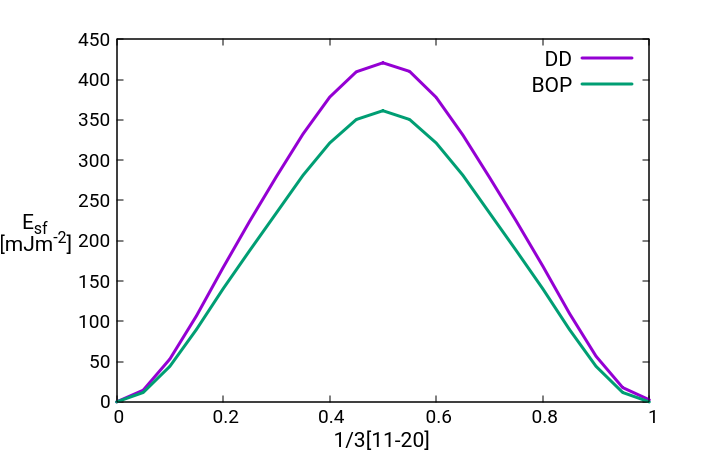
\includegraphics[width=.9\linewidth]{Images/basal_gamma_line_tbe_15_layers_bop_64_layers.png}
\end{center}

We can see that the gamma line from the bop model is consistently lower than
that of the one from the direct-diagonalisation plot. This may be due to the
fact that the number of layers in the BOP simulation was much higher (64
compared to 30), so that the actual interaction between the tight-binding
fault surfaces under homogeneous shear boundary conditions had more of an
effect on the stacking fault energy than the free surfaces in the BOP
simulation. 

\item Basal Gamma Surfaces
\label{sec:orgf831682}

\begin{enumerate}
\item tbe
\label{sec:org6dc18cf}

\begin{center}
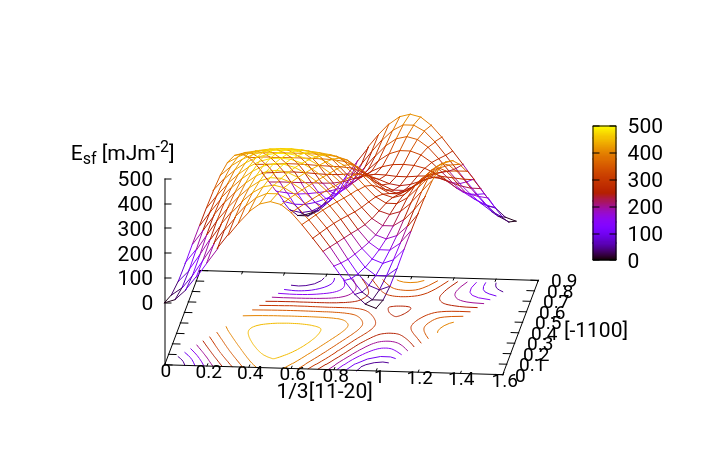
\includegraphics[width=.9\linewidth]{Images/basal_gamma_surface_tbe_15_layers_2019-09-24png.png}
\end{center}

\begin{center}
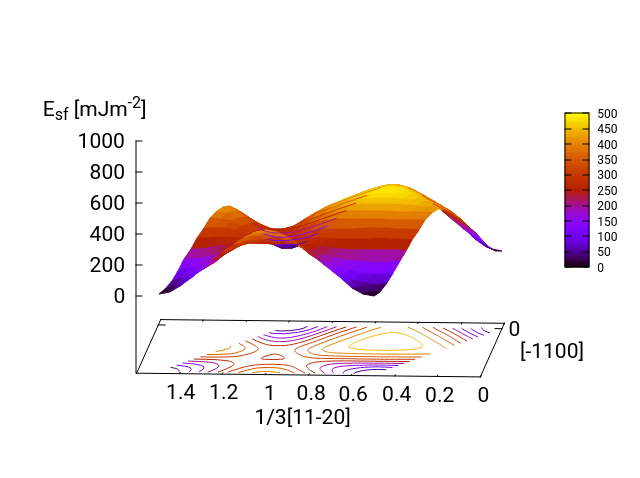
\includegraphics[width=.9\linewidth]{Images/basal_gamma_surface_tbe_15_z.png}
\end{center}
\end{enumerate}


\item Prismatic Gamma Surfaces
\label{sec:org5518551}

\begin{enumerate}
\item tbe
\label{sec:org3c53b4d}

\begin{center}
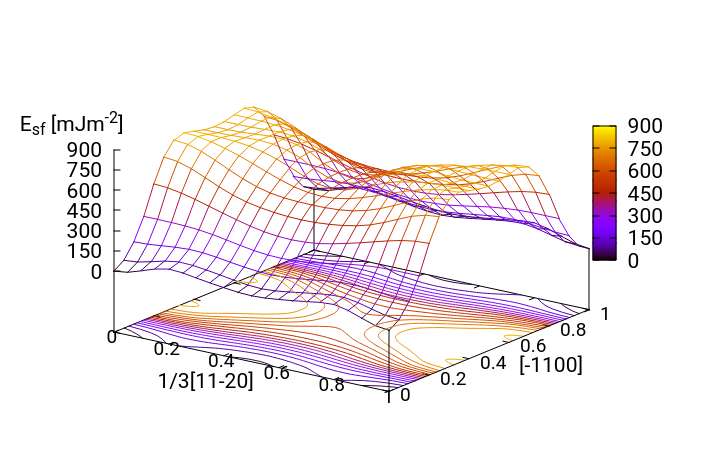
\includegraphics[width=.9\linewidth]{Images/prismatic_gamma_surface_tbe_15_layers_2019-09-24.png}
\end{center}

\begin{center}
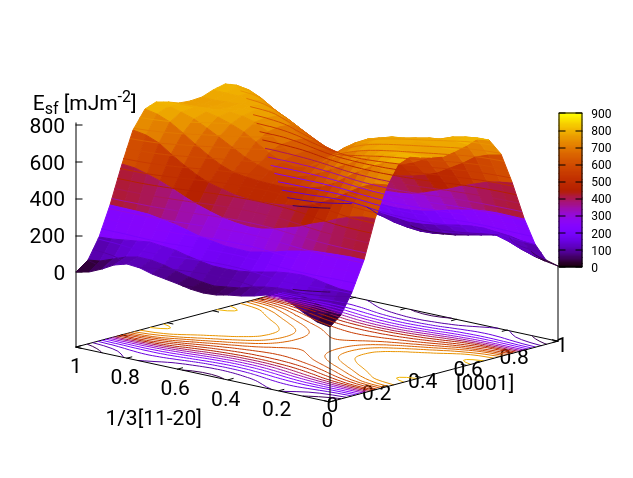
\includegraphics[width=.9\linewidth]{Images/prismatic_gamma_surface_tbe_15_z.png}
\end{center}
\end{enumerate}
\end{enumerate}

\subsection{Final Model}
\label{sec:org02c6b02}


 fdd=0.2648249504 qdds=0.5697753882 qddp=0.5648597117 qddd=0.8213593849 b0=49.75575654 p0=1.105068573 b1=-5.09734161 p1=0.6991977165 cr2=3.221758936 cr3=-1.141827235 cr1=-6.0 ndt=2.0 r1dd=6.3741123381 rcdd=9.8768388324 rmaxhm=9.9756072207 
VARGS
    -vfdd=0.2648249504 -vqdds=0.5697753882 -vqddp=0.5648597117 -vqddd=0.8213593849 -vb0=49.75575654 -vp0=1.105068573 -vb1=-5.09734161 -vp1=0.6991977165 -vcr2=3.221758936 -vcr3=-1.141827235  -vcr1=-6.0 -vndt=2.0 -vr1dd=6.3741123381 -vrcdd=9.8768388324 -vrmaxhm=9.9756072207 

a\textsubscript{hcp}   :   5.55908396   5.57678969   5.55908396   5.57678969   0.00031349 1500.00000000      4702.39
c/a     :   1.61268131   1.58731122  15.65813964  15.41181168   0.06067746 100.00000000     60677.46
a\textsubscript{omega} :   8.84739387   8.73254342   1.10592423   1.09156793   0.00020610  10.00000000        20.61
c\textsubscript{omega} :   5.38456249   5.32343103   0.67307031   0.66542888   0.00005839  10.00000000         5.84
a\textsubscript{4h}    :   5.55471471   5.56325146   0.99846551   1.00000000   0.00000235   1.00000000         0.02
c\textsubscript{4h}    :  17.98986999  17.75908031   1.01299559   1.00000000   0.00016889   1.00000000         1.69
a\textsubscript{6h}    :   5.54952123   5.54639384   1.00056386   1.00000000   0.00000032   1.00000000         0.00
c\textsubscript{6h}    :  27.05646584  26.77136353   1.01064953   1.00000000   0.00011341   1.00000000         1.13
a\textsubscript{bcc}   :   6.27665250   6.17948863   0.89666464   0.88278409   0.00019267   1.00000000         1.93
a\textsubscript{fcc}   :   7.83824788   7.88677000   1.11974970   1.12668143   0.00004805   1.00000000         0.48
DE(o,h) :  -1.09765167  -0.63343333  -0.07317678  -0.04222889   0.00095777 3000.00000000     28733.15
DE(4h,h):   1.97809750   3.17160000   0.00791239   0.01268640   0.00002279 2000.00000000       455.82
DE(6h,h):   2.97676333   3.72005000   0.01190705   0.01488020   0.00000884 2000.00000000       176.79
DE(b,h) :   9.82662500   7.63520000   0.09925884   0.07712323   0.00048999 200.00000000       979.97
DE(f,h) :   4.48794500   4.51880000   0.04533278   0.04564444   0.00000010 2000.00000000         1.94
c\textsubscript{11}    : 180.67966452 176.10000000   0.78923542   0.76923077   0.00040019 100.00000000       400.19
c\textsubscript{33}    : 206.14770273 190.50000000   0.83241552   0.76923077   0.00399231 100.00000000      3992.31
c\textsubscript{44}    :  48.30576681  50.80000000   0.73146225   0.76923077   0.00142646 100.00000000      1426.46
c\textsubscript{12}    :  95.22633084  86.90000000   0.84293468   0.76923077   0.00543227 100.00000000      5432.27
c\textsubscript{13}    :  66.46772326  68.30000000   0.74859470   0.76923077   0.00042585  50.00000000       212.92
M\textsubscript{freq}\textsubscript{0}:   2.52855122   2.85858719   0.18428037   0.20833333   0.00057855   0.10000000         0.58
M\textsubscript{freq}\textsubscript{1}:   2.52855123   2.85858719   0.18428037   0.20833333   0.00057855   0.10000000         0.58
M\textsubscript{freq}\textsubscript{2}:   2.52855123   2.85858719   0.18428037   0.20833333   0.00057855   0.10000000         0.58
M\textsubscript{freq}\textsubscript{3}:   2.52855124   2.85858719   0.18428037   0.20833333   0.00057854   0.10000000         0.58
M\textsubscript{freq}\textsubscript{4}:   5.59220819   5.66706047   0.20558160   0.20833333   0.00000757   0.10000000         0.01
M\textsubscript{freq}\textsubscript{5}:   5.59220819   5.66706047   0.20558160   0.20833333   0.00000757   0.10000000         0.01
H\textsubscript{freq}\textsubscript{0}:   3.57525560   4.80643423   0.15496829   0.20833333   0.00284783   0.10000000         2.85
H\textsubscript{freq}\textsubscript{1}:   3.57525560   5.58010025   0.13348235   0.20833333   0.00560267   0.10000000         5.60
H\textsubscript{freq}\textsubscript{2}:   6.11165910   5.65316738   0.22522990   0.20833333   0.00028549   0.10000000         0.29
H\textsubscript{freq}\textsubscript{3}:   6.11165910   6.36651842   0.19999350   0.20833333   0.00006955   0.10000000         0.07
H\textsubscript{freq}\textsubscript{4}:   7.75488320   6.40050186   0.25241781   0.20833333   0.00194344   0.10000000         1.94
H\textsubscript{freq}\textsubscript{5}:   7.75488320   7.64082373   0.21144326   0.20833333   0.00000967   0.10000000         0.01
bandw. G:   5.03138714   5.87085872   1.42835071   1.66666667   0.05679449   1.00000000       567.94
bandw. K:   6.21236174   4.97424321   1.13536901   0.90909091   0.05120178   1.00000000       512.02
bandw. M:   7.05319388   7.78109872   1.51075363   1.66666667   0.02430888   1.00000000       243.09
bandw. L:   5.72119604   6.34433701   1.50296662   1.66666667   0.02679771   1.00000000       267.98
bandw. H:   4.78240287   9.70902614   0.44779352   0.90909091   0.21279528   1.00000000      2127.95
DOSerr\textsubscript{h}:   0.00000000   0.00000000   0.00000000   0.00000000   0.00000000   0.10000000         0.00
DOSerr\textsubscript{o}:   0.00000000   0.00000000   0.00000000   0.00000000   0.00000000   0.10000000         0.00

\subsection{{\bfseries\sffamily TODO} Write first section of Literature review}
\label{sec:org5c322ff}
\subsubsection{{\bfseries\sffamily TODO} Summarise Stacking Faults and write review}
\label{sec:org75741be}
\subsubsection{{\bfseries\sffamily TODO} Write up the tight binding fitting of oxygen and an explanation for paramagnetism.}
\label{sec:orgbe45881}
\subsubsection{{\bfseries\sffamily TODO} Summarise dislocations and Oxygen interactions (review)}
\label{sec:org0f34bce}
\subsection{{\bfseries\sffamily TODO} See how the PDOS changes with addition of oxygen and how the tetrahedral/octahedral sites change this.}
\label{sec:orge23f055}
\subsection{{\bfseries\sffamily TODO} Calculate solution enthalpy of oxygen in titanium.}
\label{sec:org615de32}
\begin{itemize}
\item The solution enthalpy \(E_{\text{sol}}\) and excess volume \(\Delta V\) is 
$$ E_{\text{sol} = E( \text{Ti}_n \text{O} ) - E( \text{Ti}_n ) - E(O) $$
$$ \Delta V = V( \text{Ti}_n \text{O} ) - V( \text{Ti}_n ) $$
\item \(E( \text{Ti}_n \text{O} )\) is the excess energ of the bulk supercell with n
Ti atoms and one impurity atom. \(E( \text{Ti}_n )\) is the energy of the pure
cells.
\item Influence of cell sizes and solution enthalpy needs to be considered.
\end{itemize}

\subsection{{\bfseries\sffamily TODO} Has anyone investigated the stacking faults of Omega phase?}
\label{sec:orgc59a55e}
\begin{itemize}
\item Maybe as Omega phase doesn't occur that often, perhaps it has not been
studied in detail.
\item I should look further into thsi
\end{itemize}
\subsection{{\bfseries\sffamily TODO} Finish doing the gamma surfaces for all planes for pure titanium.}
\label{sec:org253db26}
\subsubsection{Checking the convergence criteria}
\label{sec:org77a2273}
\begin{itemize}
\item Now checking the convergence criteria.
\end{itemize}

\begin{enumerate}
\item How the lattice parameters change with the fineness of the k mesh
\label{sec:orgdaf3990}
\begin{itemize}
\item Maybe with a less fine k mesh the lattice parameters become
worse.
\item SOLUTION: The lattice parameters do not change that much under
\end{itemize}
differences with the k mesh. \href{file:///home/tigany/Documents/disl\_gsurf/hcp\_pris\_screw/hcp\_relaxed\_pris\_screw/gamma\_surfaces/get\_hom\_shear\_bc\_gs.py}{File with change of the lattice
parameters with k mesh. }
\href{file:///home/tigany/Documents/disl\_gsurf/hcp\_pris\_screw/hcp\_relaxed\_pris\_screw/gamma\_surfaces/a\_hcp\_vs\_nk.png}{a vs nk}
\href{file:///home/tigany/Documents/disl\_gsurf/hcp\_pris\_screw/hcp\_relaxed\_pris\_screw/gamma\_surfaces/c\_hcp\_vs\_nk.png}{c\textsubscript{vs}\textsubscript{nk}}
\href{file:///home/tigany/Documents/disl\_gsurf/hcp\_pris\_screw/hcp\_relaxed\_pris\_screw/gamma\_surfaces/e\_hcp\_vs\_nk.png}{e\textsubscript{vs}\textsubscript{nk}}

\begin{enumerate}
\item What if rmaxh is smaller or larger?
\label{sec:org0fafb30}
\begin{itemize}
\item If rmaxh is is smaller (say rmaxh = 6.7 bohr) then we get the same
results.
\end{itemize}
\begin{figure}[htbp]
\centering
\includegraphics[width=.9\linewidth]{/home/tigany/Documents/disl_gsurf/hcp_pris_screw/hcp_relaxed_pris_screw/gamma_surfaces/e_hcp_vs_nk_small_rmaxh_better_format.png}
\caption{\label{fig:orgaf41d69}
Variation of energy with k mesh.}
\end{figure}
\begin{figure}[htbp]
\centering
\includegraphics[width=.9\linewidth]{/home/tigany/Documents/disl_gsurf/hcp_pris_screw/hcp_relaxed_pris_screw/gamma_surfaces/a_hcp_vs_nk_small_rmaxh_better_format.png}
\caption{\label{fig:org8c2dd2a}
Variation of a hcp with k mesh.}
\end{figure}
\begin{figure}[htbp]
\centering
\includegraphics[width=.9\linewidth]{/home/tigany/Documents/disl_gsurf/hcp_pris_screw/hcp_relaxed_pris_screw/gamma_surfaces/c_hcp_vs_nk_small_rmaxh_better_format.png}
\caption{\label{fig:org3a41bbf}
Variation of c hcp with k mesh.}
\end{figure}]]
\begin{itemize}
\item Data: \href{file:///home/tigany/Documents/disl\_gsurf/hcp\_pris\_screw/hcp\_relaxed\_pris\_screw/gamma\_surfaces/a\_hcp\_vs\_nk\_rmaxh\_small.pkl}{a\textsubscript{hcp} small rmaxh}, \href{file:///home/tigany/Documents/disl\_gsurf/hcp\_pris\_screw/hcp\_relaxed\_pris\_screw/gamma\_surfaces/c\_hcp\_vs\_nk\_rmaxh\_small.pkl}{c\textsubscript{hcp} small rmaxh}, \href{file:///home/tigany/Documents/disl\_gsurf/hcp\_pris\_screw/hcp\_relaxed\_pris\_screw/gamma\_surfaces/e\_hcp\_vs\_nk\_rmaxh\_small.pkl}{e\textsubscript{hcp} small rmaxh}.
\end{itemize}
\begin{itemize}
\item If rmaxh is larger ( rmaxh = 20 bohr ), all possible interactions must
be included then. And so we get the same results.
\end{itemize}
\begin{figure}[htbp]
\centering
\includegraphics[width=.9\linewidth]{/home/tigany/Documents/disl_gsurf/hcp_pris_screw/hcp_relaxed_pris_screw/gamma_surfaces/e_hcp_vs_nk_large_rmaxh.png}
\caption{\label{fig:org02e440e}
Variation of energy with k mesh.}
\end{figure}
\begin{figure}[htbp]
\centering
\includegraphics[width=.9\linewidth]{/home/tigany/Documents/disl_gsurf/hcp_pris_screw/hcp_relaxed_pris_screw/gamma_surfaces/a_hcp_vs_nk_large_rmaxh.png}
\caption{\label{fig:orgfbc824f}
Variation of a hcp with k mesh.}
\end{figure}
\begin{figure}[htbp]
\centering
\includegraphics[width=.9\linewidth]{/home/tigany/Documents/disl_gsurf/hcp_pris_screw/hcp_relaxed_pris_screw/gamma_surfaces/c_hcp_vs_nk_large_rmaxh.png}
\caption{\label{fig:org630882a}
Variation of c hcp with k mesh.}
\end{figure}
\begin{itemize}
\item Data: \href{file:///home/tigany/Documents/disl\_gsurf/hcp\_pris\_screw/hcp\_relaxed\_pris\_screw/gamma\_surfaces/a\_hcp\_vs\_nk\_rmaxh\_large.pkl}{a\textsubscript{hcp} large rmaxh}, \href{file:///home/tigany/Documents/disl\_gsurf/hcp\_pris\_screw/hcp\_relaxed\_pris\_screw/gamma\_surfaces/c\_hcp\_vs\_nk\_rmaxh\_large.pkl}{c\textsubscript{hcp} large rmaxh}, \href{file:///home/tigany/Documents/disl\_gsurf/hcp\_pris\_screw/hcp\_relaxed\_pris\_screw/gamma\_surfaces/e\_hcp\_vs\_nk\_rmaxh\_large.pkl}{e\textsubscript{hcp} large rmaxh}
\end{itemize}
\end{enumerate}

\item How does rmaxh change the lattice parameters?
\label{sec:org7b8d288}

\begin{enumerate}
\item How does rmaxh change the energy of a supercell
\label{sec:orgf019641}
\begin{itemize}
\item How does the number of neighbours change and what is the relation
between rmaxh and larger cell sizes.
\end{itemize}
\end{enumerate}
\end{enumerate}
\subsubsection{Notes on the model.}
\label{sec:org449a6fa}
It seems that there is a lot of charge moving around when doing the
relaxations. 
I think that this may be due to the fact that there is no Hubbard U
interactions, a parameter for the coulomb interaction, which stops the
charges from moving freely. 
\begin{itemize}
\item TBE control file is currently set to this:
\begin{minted}[]{bash}
TBE: nbas = 128 nspec = 1 verb 31 
TB: rmaxh = 20, m-stat: F-P rlx-vol, rho 
bz: metal
\end{minted}
\end{itemize}



\subsubsection{{\bfseries\sffamily DONE} Implement Homogenous Shear boundary conditions for gamma surface calculation.}
\label{sec:org30db119}
\section{Notes}
\label{sec:orgf304a93}
\subsection{Dislocation dipole simulation}
\label{sec:org804f94f}

\textit{<2019-03-29 Fri>}
It seems that actually, for the Clouet method, the \emph{x} component for the
accomodaton of strain is \emph{positive}. These additions to the tilt vectors make
the dislocatons in a stable position in the quadrupolar array. 

There is no asymmetry in relaxations now between the dislocations of different
sign. This now works as expected. 




\subsection{Embedded atom method}
\label{sec:orga25c3e6}
This is a semi empirical method that does not take into account directional
bonding. It does not treat covalency or charge transfer. Neither does it
incorporate Fermi surface effects. 

The main physical property incorporated in the EAM is the moderation of bond
strength by other bonds (coordination-dependent bond strength).

\section{Completed Tasks\hfill{}\textsc{ARCHIVE}}
\label{sec:org2082c82}

\section{Bibliography}
\label{sec:orga525d4a}
\label{org937368d}

\bibliographystyle{unsrt}
\bibliography{bibliography/org-refs}

\section{Current Papers}
\label{sec:org35f3849}

\subsection{Omega phase transformation – morphologies and mechanisms.}
\label{sec:org0a405f5}
Banerjee, S., Tewari, R., \& Dey, G. K. (2006). 
International Journal of Materials Research, 97(7),
963–977. \href{https://doi.org/10.3139/146.101327}{doi:10.3139/146.101327} 
\cite{Banerjee_2006}


Omega is found in both trigonal and perfect (hexagonal) forms. 

Positions are:
A: 0. 0. 0. 
B: 2/3 1/3 (1/2-z); 1/3 2/3 (1/2+z)

Where z = 1/6 is cubic symmetry. 

The two atomic sites in the omega unit cell are not equivalent.  B-type atomic
sites are more closely packed as compare to the A-type atomic site.
\end{document}
